%----------------------------------------------------------------------------------------
%	PACKAGES AND OTHER DOCUMENT CONFIGURATIONS
%----------------------------------------------------------------------------------------
\documentclass[11pt, english, singlespacing, headsepline]{classes/ResearchTopic}

\usepackage[utf8]{inputenc} % Required for inputting international characters
\usepackage[T1]{fontenc} % Output font encoding for international characters
\usepackage{mathpazo} % Use the Palatino font by default
\usepackage{todonotes}

\newcommand{\hajj}[2][]{\todo[inline, color=green, author=elhajj, #1]{#2}}
% \usepackage[backend=bibtex,style=authoryear,natbib=true]{biblatex} % Use the bibtex backend with the authoryear citation style (which resembles APA)

\usepackage[%
    style=ieee, %apa of ieee?
    isbn=false,
    url=false,
    doi=true
]{biblatex}
\addbibresource{references.bib} % The filename of the bibliography

\usepackage[autostyle=true]{csquotes} % Required to generate language-dependent quotes in the bibliography
\usepackage{nicematrix} % For Nicetabular table
\usepackage{calc}
% for multiple citation reference
% \usepackage{cite} 
% for managing images and figures
\usepackage{graphicx}
% For alligning table caption
\usepackage{caption}
\newcolumntype{P}[1]{>{\raggedright\arraybackslash}p{#1\textwidth-2\tabcolsep-1.5\arrayrulewidth}}
\newcolumntype{Y}[1]{>{\centering\arraybackslash}p{#1\textwidth-2\tabcolsep-1.5\arrayrulewidth}}
\usepackage{tcolorbox} % for shadwo box 
\usepackage{svg} % for svg 
\usepackage[export]{adjustbox} % to possition image and table
\usepackage{parskip} % to disable automatic indentation and provid space between pargarphs 
\usepackage{floatrow} % to put table label and caption above the table 
\usepackage{threeparttable} % to put table label and caption above the table
%----------------------------------------------------------------------------------------
%	MARGIN SETTINGS
%----------------------------------------------------------------------------------------

\geometry{
	paper=a4paper, % Change to letterpaper for US letter
	inner=3.0cm, % Inner margin
	outer=3.8cm, % Outer margin
	bindingoffset=0.5cm, % Binding offset
	top=1.5cm, % Top margin
	bottom=1.5cm, % Bottom margin
	%showframe, % Uncomment to show how the type block is set on the page
}

%----------------------------------------------------------------------------------------
%	THESIS INFORMATION
%----------------------------------------------------------------------------------------

\thesistitle{Digital Twin and Securing IoT applications} % Your thesis title, this is used in the title and abstract, print it elsewhere with \ttitle
\supervisor{Dr.Ing M.Mohammed\textsc{Elhajj}} % Your supervisor's name, this is used in the title page, print it elsewhere with \supname
\examiner{} % Your examiner's name, this is not currently used anywhere in the template, print it elsewhere with \examname
\degree{Master of Computer Science} % Your degree name, this is used in the title page and abstract, print it elsewhere with \degreename
\author{Teklit \textsc{Haphtu}} % Your name, this is used in the title page and abstract, print it elsewhere with \authorname
\addresses{} % Your address, this is not currently used anywhere in the template, print it elsewhere with \addressname

\subject{Cybersecurity, Computer Science} % Your subject area, this is not currently used anywhere in the template, print it elsewhere with \subjectname
\keywords{Digital Twin, Internet of Things, authentication} % Keywords for your thesis, this is not currently used anywhere in the template, print it elsewhere with \keywordnames
\university{\href{http://www.utwente.nl}{University of Twente}} % Your university's name and URL, this is used in the title page and abstract, print it elsewhere with \univname
\department{\href{http://department.university.com}{Department of Computer Science}} % Your department's name and URL, this is used in the title page and abstract, print it elsewhere with \deptname
\group{\href{https://www.utwente.nl/en/eemcs/scs/}{Service And Cybersecurity (SCS)}} % Your research group's name and URL, this is used in the title page, print it elsewhere with \groupname
\faculty{\href{https://www.utwente.nl/en/eemcs/}{EEMCS}} % Your faculty's name and URL, this is used in the title page and abstract, print it elsewhere with \facname

\AtBeginDocument{
\hypersetup{pdftitle=\ttitle} % Set the PDF's title to your title
\hypersetup{pdfauthor=\authorname} % Set the PDF's author to your name
\hypersetup{pdfkeywords=\keywordnames} % Set the PDF's keywords to your keywords
}


\begin{document}

\frontmatter % Use roman page numbering style (i, ii, iii, iv...) for the pre-content pages

\pagestyle{plain} % Default to the plain heading style until the thesis style is called for the body content

%----------------------------------------------------------------------------------------
%	TITLE PAGE
%----------------------------------------------------------------------------------------

\begin{titlepage}
\begin{center}

\vspace*{.06\textheight}
{\scshape\LARGE \univname\par}\vspace{1.5cm} % University name
\textsc{\Large Master of Computer Science}\\[0.5cm] % Thesis type

\HRule \\[0.4cm] % Horizontal line
{\huge \bfseries \ttitle\par}\vspace{0.4cm} % Thesis title
\HRule \\[1.5cm] % Horizontal line
 
\begin{minipage}[t]{0.4\textwidth}
\begin{flushleft} \large
\emph{Author:}\\
\href{http://www.teklithaphtu.com}{\authorname} % Author name - remove the \href bracket to remove the link
\end{flushleft}
\end{minipage}
\begin{minipage}[t]{0.4\textwidth}
\begin{flushright} \large
\emph{Supervisor:} \\
\href{https://people.utwente.nl/m.elhajj}{\supname} % Supervisor name - remove the \href bracket to remove the link  
\end{flushright}
\end{minipage}\\[3cm]
 
\vfill

\large \textit{A thesis submitted in fulfillment of the requirements\\ for the degree of \degreename}\\[0.3cm] % University requirement text
\textit{in the}\\[0.4cm]
\groupname\\\deptname\\[2cm] % Research group name and department name

\vfill

{\large \today}\\[4cm] % Date
%\includegraphics{Logo} % University/department logo - uncomment to place it
 
\vfill
\end{center}
\end{titlepage}


%----------------------------------------------------------------------------------------
%	THESIS CONTENT - CHAPTERS
%----------------------------------------------------------------------------------------

\mainmatter % Begin numeric (1,2,3...) page numbering

\pagestyle{thesis} % Return the page headers back to the "thesis" style

% Include the chapters of the thesis as separate files from the Chapters folder

% Chapter 1

\chapter{Introduction} % Main chapter title

\label{Chapter1} % For referencing the chapter elsewhere, use \ref{Chapter1} 

%----------------------------------------------------------------------------------------
% Define some commands to keep the formatting separated from the content 
\newcommand{\keyword}[1]{\textbf{#1}}
\newcommand{\tabhead}[1]{\textbf{#1}}
\newcommand{\code}[1]{\texttt{#1}}
\newcommand{\file}[1]{\texttt{\bfseries#1}}
\newcommand{\option}[1]{\texttt{\itshape#1}}

%----------------------------------------------------------------------------------------
% 
% \hajj{Chapter One introduces the topic of the thesis to the reader. The critical part of writing Chapter One is to establish the statement of the problem and research questions. Basically, you are justifying to the reader why it is nec- essary to study this topic and what research question(s) your study will answer. Usually, the topic is based around a particular problem area that you want to focus on. However, before you introduce the reader to the specific topic and problem, you have to first provide the reader with the broader context (the general problem) and consequences related to the topic. In other words, before you discuss the specific problem, you need to contextualize your topic within the larger problem. For example, you would first discuss the problems related to the topic.
% Chapter One of the thesis includes a section on the Statement of the Problem (information about the specific problem), Background and Need (the background literature related to the problem), the Purpose of the Study (the focus and goal of the study), Research Questions (what questions the study proposes to answer), and other significant sections. In this chapter, you need to support all of your claims and positions using citations
%  check this reference please:
%  https://www.wcupa.edu/business-publicManagement/geographyPlanning/documents/thesisGuideline.pdf}
% \begin{enumerate}
    %item state the general topic and give some background
    %\item provide a review of the literature related to the topic
        % \item define the terms and scope of the topic
        % \item outline the current situation
        % evaluate the current situation (advantages/ disadvantages) and identify the gap
    % \item identify the importance of the proposed research
    % \item state the research problem/ questions
    % \item state the research aims and/or research objectives
    % \item state the hypotheses. DONE
    % \item outline the order of information in the thesis. DONE
    % \item outline the methodology. DONE
% \end{enumerate}


% General Research topic 
\textbf{Research Topic}:
% Data exchange and connectivity 
% Sensors and actuators 
% Industrial process is becoming intelligent through digital twin
% Machines are communicating with each other to get data for processing 
% 
% We are in an era where it is difficult for industries and organisations to operate without connectivity and data exchange. With the advent of Industry 4.0, Digital Twins(DT) and Internet of Things(IoT) are the two enabling technologies that provide unprecedented levels of connectivity and data exchange to monitor and optimise business operation. Both technologies have been around for a while, but the integration of of them is just getting started.
Connectivity and data exchange are two of the characteristics of Industry 4.0. Industrial Internet of Things ((I)IoT) sensors are a vital component of this paradigm, facilitating the collection and transmission of environmental data from the physical system to the central station for processing and analysis(Digital Twin). However, although sensors play a critical role in this process, they are not inherently equipped to run strong encryption mechanisms to secure the data they transmit over wired or wireless channels. This research aims to explore the security challenges posed by power and storage limitations of (I)IoT sensors in the application of Digital Twin within Industry 4.0 use cases. 



% \textbf{Literature Review}:
% % Methodology Summary 
% % The core concept of Digital Twin
% % How digital twin is used to securing IoT application 
% % How data is secure 
% This study conducted a systematic literature review to investigate the use of Digital Twin in enhancing the security of IoT applications in industry 4.0. The review followed a three-phase approach, including the use of automated tools for the review process. A total of 523 papers were initially collected from seven digital libraries, and after applying inclusion and exclusion criteria and quality assessment, 56 relevant papers were selected for review. 

% The definition of digital twins in the literature varies depending on the context, but generally, it consists of three components: physical and digital states, interconnectivity, and a process for collecting and examining data.

% The use cases for digital twins are vast, including threat detection and response, vulnerability assessment, security awareness training, and threat intelligence. A wide range of industry 4.0 sectors benefit from this technology, including the power grid, automotive industry, water treatment plants, transportation systems, and satellite internet, among others. Researchers have deployed security-enabled digital twins to improve the security and safety of operations.  
% Machine learning and data analytics are the two primary technologies widely used by study authors to enable digital twin security features. Other technologies, such as blockchain, cloud computing, and federated learning, are also used. However, most authors neglect the security concerns related to the data used by digital twins during transmission and while at rest.  
% Some researchers have proposed encryption methods, such as AES and RSA, to secure digital twin data. However, these methods may not be feasible for deployment in device-constrained devices. Other researchers have suggested using blockchain to maintain the integrity and reliability of data shared by a network of digital twins.  

\textbf{Niche and Scope}:
% Industry 4.0 smart manufacturing, 
% IIoT application 
% Digital Twin use case
% 
The (Industrial) Internet of Things is a system of interconnected physical devices, such as sensors and actuators, that are embedded in technology to allow the communication and exchange of data through wireless networks \cite{maillet-contozEndtoendSecurityValidation2020}. The adoption of Industrial Internet of Things (IIoT) in industrial settings aims to improve efficiency, productivity, and safety by gathering and analyzing data from connected devices, sensors, and machines \cite{kumarBlockchainDeepLearning2022}. However, the gap between enterprise Information Technology (IT) and Operational Technology (OT) has been a challenge in implementing (I)IoT due to different standards, protocols, and security requirements \cite{adrienbacueDigitalTwinsEnhanced2022}.

Digital Twin, on the other hand, is software-defined digital representation of physical object that operate on a large set of environmental sensor data to simulate and monitor operation in real-time \cite{williamdanilczykANGELIntelligentDigital2019, danilczykSmartGridAnomaly2021}. Simulation of an operation, visualization of product in real-time, troubleshooting remote equipment \cite{alcarazDigitalTwinComprehensive2022, veledarDigitalTwinsDependability2019, vargheseDigitalTwinbasedIntrusion2022}, and managing assets in industry are a few of the use cases among the others. Together, those two technologies are transforming the way we manage resources and operations in various industry use cases.


% The importance of this research
% The challenge in storytelling scenario 
\textbf{Importance of the Research}:
Digital Twin and (I)IoT technologies have recently emerged to play important roles across various industries, including aerospace engineering, electric grid, car manufacturing, petroleum industry, healthcare, and more \cite{tao_digital_2018}. For these technologies to function properly in an industrial setting, authentic and un corrupted data \cite{fuller_digital_2020} in real-time is required \cite{yuchenziqianzhangningtangApplicationDigitalTwin2022}. 

However, in most cases, the data transmitted over wired or wireless from the source ((I)IoT) to the central processing station (DT) is vulnerable to a variety of cyber threats, such as eavesdropping, tampering, and replay attacks \cite{hussainiTaxonomySecurityDefense2022}. These attacks can result in the unauthorized access, modification, or theft of sensitive data, potentially causing significant harm to organizations that rely on these technologies.

Therefore, it is critical to secure the data channels used for interaction and communication between DT  and (I)IoT technologies to ensure the integrity and authenticity of data. Authentication is a fundamental security principle that can address this concern by allowing only authorized endpoints to access and consume data. In the context of DT and (I)IoT, authentication can help ensure that only known (I)IoT devices can send sensor data to the DT hub and only known Digital Twins can send commands to remote devices. In addition to authentication, other security measures, such as encryption and data integrity checks, can be employed to further strengthen the security of DT and (I)IoT applications.

Further, in industry 4.0 use cases, (I)IoT devices, such as sensors and actuators, are typically located in remote areas that are difficult to access. As a result, it is also crucial to implement an efficient and reliable cryptographic solution that can increase the lifespan of these power-constraint devices and avoid frequent repairs or replacements.     


% Problem statement 
\textbf{Problem Statement}:
As noted previously, manufacturing facilities, including critical infrastructure, are using an (I)IoT devices to collect and send sensor measurements and operating conditions to the Digital Twin station to monitor and optimize the overall operation of the business process. However, due to the storage and processing constraints that (I)IoT devices have \cite{williams_survey_2022,noauthor_lightweight_nodate}, it is challenging to adopt traditional cryptographic security mechanisms to ensure the confidentiality and integrity of the data flow between (I)IoT and DT. If proper security measures (authentication, authorization, encryption, and so on) are not used, an attacker may be able to perform a man-in-the-middle attack with the intent of intercepting sensitive sensor data or disrupting a system by injecting crafted faulty data \cite{salimBlockchainEnabledSecureDigital2022}. In recent literatures and blog of standard institutes, it is mentioned to utilize security schemes that can fit into constraint devices to address the security requirement.  

% Proposed Solution and Hypothesis 
\textbf{Proposed Solution}:
The National Institute of Standards and Technology (NIST) has developed a set of standards for lightweight cryptography that are designed to provide cryptographic security with limited storage and computing resources, such as those found in small devices like sensors or smart cards.

In this study, we propose an authentication/encryption scheme based of one of the NIST standard lightweight cryptography algorithms. According to NIST \cite{noauthor_lightweight_nodate}, the algorithms have a small code size and low power consumption, while still providing a high level of security.  This NIST-standardised lightweight-based authentication scheme will enhance the confidentiality and integrity of data exchanged via the communication channel between the DT and its counter-physical component.


\textbf{Research Objective and Aims}:
The aim of this research is two-fold. First, conduct a systematic literature review to analyze the concept of Digital Twins and how they can enhance the security of IIoT/IoT applications in industry 4.0 use cases. Secondly, to implement a NIST standard lightweight authentication scheme to improve the security of digital communication between power, storage, and processing constraint devices and DT stations hosted on cloud or local premises.


\textbf{Hypothesis}:
% More security
% efficiency increases speed of data flow 
% Getting a real-time of data is one requirement of the DT application 
Implementing a lightweight encryption/authentication scheme based on the NIST standard can enhance the security and integrity of data flow between DT and power constraint (I)IoT sensors. This solution can reduce memory footprint, power consumption, and latency. 

The proposed solution in this paper-implementing ligthweight based authentication- can facilitate the secure exchange of data between DT and IIoT sensors while preventing unauthorized access to sensitive information. The scheme utilises symmetric key cryptography, which is computationally efficient and suitable for power-constrained devices while supporting mutual authentication to verify the identities of both the DT and the IIoT sensors before exchanging data.



The proposed scheme utilizes symmetric key cryptography, which is computationally efficient and suitable for power-constrained devices. 

It supports mutual authentication to verify the identities of both the DT and the IIoT sensors before exchanging data, thus preventing unauthorized access to sensitive information.



% Methodology 
\textbf{Methodology}:
This study has two major parts; literature review and implementation of the proposed solution. For the literature review, we conducted a systematic way of reviewing previous literatures with the aim of synthesizing the concept of Digital Twin and analyzing how Digital Twin is used to secure IoT applications with in industry 4.0 use case. 

To implement our proposed solution, which is a lightweight authentication scheme, we leverage a 
Digital Twin open-source platform called Ditto and one of ESP32 family microcontrollers from Espressif systems.As we mentioned before Ditto is an open-source software design patter, developed and maintained by Eclipse Foundation to facilitate the integration  Digital Twin and IoT devices\cite{noauthor_eclipse_nodate}. On the other hand, ESP32 popular microcontrollerchip used in IoT application. It has low power consumption, WiFi and Bluetooth connectivity and a wide range of peripheral interfaces.  

In addition, the performance and efficiency of our proposed solution are compared with the traditional  method of providing encryption and authentication mechanisms by measuring the power consumption, execution time, and storage complexity. 
% The following diagram provides the general setting of our proposed solution.

% \begin{figure}[H]
%     \label{fig:ps-scheme}
%     \caption{General Setting of Proposed Solution}
%     \centering
%     \includesvg[width=\textwidth]{images/svg/ps-scheme-final.svg}
    
% \end{figure}

% outline the order of information in the thesis 
\textbf{Report outline}:
The remainder of this study report is organized as follows. In the following section, we present the methodology we employed for the systematic literature review process. Then we provide details results of the literature review. Following that, we discuss the summary of the result and limitations of the study. Finally, we draw our conclusion on the basis of the evidence we gathered.   


% Chapter 2
\chapter{Literature Review Methodology} % Main chapter title

\label{Chapter2} % For referencing the chapter elsewhere, use \ref{Chapter1} 

In this study, we plan to address half of the research questions through a literature review. Hence, we decided to follow a structured and systematic way of reviewing literature. 

A systematic literature review is one type of literature review that has a formal and structured procedure to synthesize the knowledge of existing research studies that are relevant to answer a pre-defined research questions \cite{kofod-petersen_how_nodate, kitchenham_guidelines_2007}. It allow us to understand the current state of the literature and identify research gaps\cite{carrera-rivera_how-conduct_2022}. 

This systematic literature review has two main objectives. First, to identify existing solutions that leverage Digital Twin to enhance security principles for IoT applications. As an extension and subsection of this objective, the concrete concept of the Digital Twin will be synthesised on the way. Second, to identify research studies conducted on the matter of establishing a secure communication channel between Digital Twin and Iot through cryptographic authentication mechanisms.  

We adopted Kitchenham and Charter three phases of performing systematic literature review; namely, planning protocol, conducting review, and reporting review. Basing this guideline and other resources, we created flow diagram for conducting review review process. The flow diagram of the scheme is depicted in Figure \ref{fig:slr-proc}. 

\begin{figure}[h!]
    \centering
    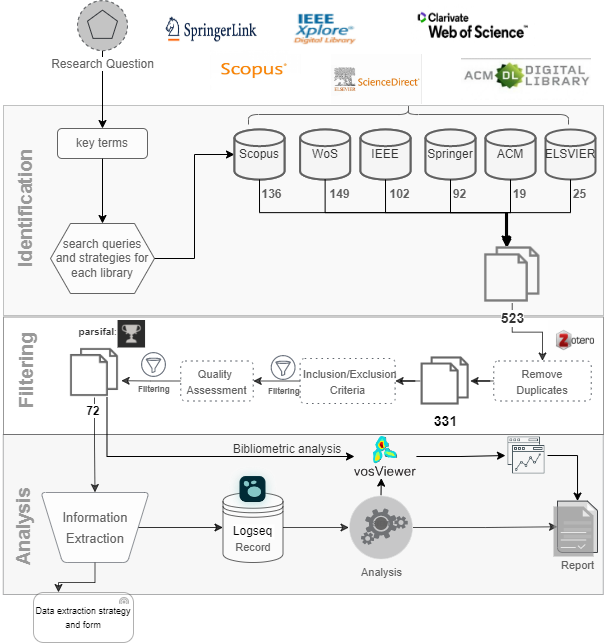
\includegraphics[width=1\textwidth]{images/slrmethoddiagram_v2.png}
    \caption{Scheme of 2nd stage (conducting review) }
    \label{fig:slr-proc}
\end{figure}


To automate the systematic literature review process, from defining the PICOC to data extraction, we use a web tool called \textit{parsif.al}\footnote{\href{https://parsif.al}{Parsifal} is an online tool designed to support researchers in performing systematic literature reviews within the context of software engineering. Geographically distributed researchers can work together within a shared workspace, designing the protocol and conducting the research}

\section{Review Protocol}

% \subsection{PICOC and Synonyms}
%----------------------------------------------------------------------------------------
% ======================================================================================================
% NOTES, TODOS
% ======================================================================================================

\subsection{Defining PICOC}
PICOC stands for Population, Intervention, Comparison, Output and Context. It is a widely used technique in medical and social science studies to define the focus of a research \cite{carrera-rivera_how-conduct_2022}. However, Kitchenham and Charter  in \cite{carrera-rivera_how-conduct_2022} and Carrera in \cite{kitchenham_guidelines_2007} showed that this technique can also be applied for computer science related research to formulate and structure research questions. 

In this subsection, we define our PICOC criteria for this systematic literature review as follow:-

\textit{Population:} The motivation to conduct this research is the security related problem we identified in the communication between Digital Twin and constrained  (I)IoT devices deployed in the smart industry to collect sensor data. Hence, the problem domain or "Population" for this research is (I)IoT devices used with Digital Twin to enhance security in Industry 4.0. Industries that use Digital Twin and (I)IoT devices, such as smart cities, smart homes, smart grids, smart health, smart manufacturing, etc. In this sense, the "Population" part of PICOC in this review refers to the following terms: Digital Twin, (Industrial)Internet of Things, Industry 4.0, Smart Manufacturing, Cyber-physical Systems, and Critical Infrastructure. 

\textit{Intervention:} Our intervention to address the aforementioned problem - the security issue of digital communication between Digital Twin and (I)IoT - is to implement a lightweight NIST standard cryptographic authentication/encryption scheme for power, storage and computation constraint (I)IoT devices. In this regard, we use the term "authentication" as an intervention.

\textit{Comparison:} Before designing and implementing an intervention for a specific problem, it is important to identify the existing solution in the literature. The results of reviewing, comparing and analysing the existing solution discussed in the relevant research literature can be used as input to design and implement the intervention methodology. With this regard, this study will identify and compare authentication schemes or security mechanisms used in securing a data flow between Digital Twin and (I)IoT. 

\textit{Outcome:} This study has two broad categories of outcomes. The expected outcome of the literature review is to provide insight into the potential benefits of DT in securing (I)IoT applications in Industry 4.0. From a technical implementation perspective, the expected outcome is a bidirectional secure remote access between DT and (I)IoT and ensuring data integrity and a secure communication channel with an efficient and performant cryptographic authentication and encryption scheme for constrained devices.\\

\textit{Context:} This systematic literature review is focused on the Industry 4.0 environment, targeting Digital Twin solutions deployed in smart industries to enhance security. On the other hand, the second part of this study is focused on implementing authentication/encryption algorithms in constrained physical device to measure and compare the performance of lightweight and traditional algorithms in terms of power consumption, execution time and memory usage. 
%----------------------------------------------------------------------------------------


% \subsection{Research Questions}
%----------------------------------------------------------------------------------------
% ======================================================================================================
% NOTES, TODOS
% ======================================================================================================

\subsection{Research Question}
Before beginning the process of study identification and data extraction, it is crucial to identify and clearly define a research question or objectives, as they serve as the guiding principles for conducting a literature review\cite{carrera-rivera_how-conduct_2022}. This systematic literature review aims to address the following research questions:

\begin{itemize}

    % RQ1
    \item \textbf{RQ1: How is Digital Twin used to enhance the security of IoT/IIot applications in the industry 4.0 use cases ?} - 
    this question aims to identify how Digital Twin is used to improving the security of industries that use IoT devices including sensors and actuators to achieve OT (operational technology) security goals: Safety, reliability and availability.
    % \begin{itemize}
    %     % I need a comment from Mohammed on this -> with regad to use case -> is to braod and vogue?
    %     \item \textbf{RQ1.1: What is the concrete concept of Digital Twin} - 
    %     under subcategory of the above research question, the concept of digital and its use cases are explored.
    % \end{itemize}

    % RQ 1
    % \item RQ1. What mututal authentication schemes for DT and IoT application are discussed in the literature? 
    % \item How can we use Digital Twin to enhance security issue in IoT/IIoT application? 
    %  Replace schemes by  mechansims.
    \item \textbf{RQ2: What are the security schemes presented in the literature to ensure the authentication between Digital Twin and its mapped physical devices?} - 
    this question focuses on the identification of authentication mechanisms that are used to ensure the security of DT and (I)IoT communication.
\end{itemize}
%----------------------------------------------------------------------------------------

% \subsection{Key Terms and Search Strategy}
%----------------------------------------------------------------------------------------
% ======================================================================================================
% NOTES, TODOS
% ======================================================================================================
% Define the search strategy for each database if possible 
% Also prepare table with or and operators refer poatek
% I need to modify the title and the resarch question -> Iot to IIoT , the area is in manufcturing or Industry 4.0.
% receive comment on the keyword variants. example IIoT, schemes.
% =======================================================================================================
\subsection{Search keys and Strategies}
Guided by the PICOC criteria and  research questions, we construct four main search strings to create search queries used for each selected databases. These are, "Digital Twin" "IoT" "Authentication", and "Industry". Synonyms, alternative spellings, and similar semantic meanings are considered for each keyword and combined using OR operator. 

During pilot search, on majority of databases, we identified that adding synonyms of "Digital Twin" does not return new paper compared to searching using only the term "Digital Twin". Even though, we included the synonym terms in the table below, we avoided using them during query construction to simplify our search string. 

\begin{table}[h]
% \captionsetup{
%   justification=raggedright,
%   singlelinecheck=false,
%   margin=60pt % adjust margin as needed
% }
% \centering
\caption{ Key terms and key variants.}
\begin{NiceTabular}{p{3.2cm}p{11cm}}
\toprule
    \textbf{Key terms} & \textbf{Variants / Synonyms / Similar Semantic Meaning} \\
    \midrule
    Digital Twin & DT, digital-twin, digital-twins, digital replica, digital shadow, virtual model, virtual clone \\ \hline
    (Industrial)Internet of Things & IoT, IIoT, internet-of-things, internet-of-thing, industrial internet of things, industrial-internet-of-thing, sensors, actuators, smart devices  \\ \hline
    Authentication & security, confidentiality, certificate, verification, scheme, schemes\\ \hline
    Industry & industry 4.0, manufacturing, smart manufacturing, factory, smart factory, cyber-physical system, cyber-physical systems, cyber physical systems, cyber physical system, critical infrastructure, critical infrastructures. \\ 
\bottomrule
\end{NiceTabular}
\end{table}

% As an example, an advance search query for Scopus databases is shown in table \ref{}.\\


% \begin{table}[h]
% % \centering
% \caption{\label{scopus-advanc-search} Example of advanced search query in Scopus}
% \begin{NiceTabular}{Y{1.1}}
% \CodeBefore
%   \rowcolor{gray!50}{1}
%   \rowcolors{2}{gray!25}{white}
% \Body
%  ("dt" OR "digital twin" OR "digital twins" OR "digital-twin" OR "digital-twins" OR "digital replica" OR "digital shadow" OR "virtual model" "virtual clone")  \\
%  AND \\
%  ("internet of things" OR "internet of thing" OR "internet-of-thing" OR "internet-of-things" OR "IIoT" OR "industrial internet of things" OR "industrial-internet-of-thing" OR "sensors" OR "actuators" OR "smart devices" )  \\
%  AND \\
% ("security" OR "authentication" OR "certificate" OR "verification" OR "schemes") \\
%  AND \\
% ("industry" OR "industry 4.0" OR "manufacturing" OR "smart manufacturing" OR "factory" "smart factory" OR "cyber-physical systems" OR "cyber-physical system" OR "cyber physical system")  \\
% \end{NiceTabular}
% \end{table}
%----------------------------------------------------------------------------------------

% \subsection{Digital Library}
%----------------------------------------------------------------------------------------
% ======================================================================================================
% NOTES, TODOS
% ======================================================================================================
% One paragraph about the databases 
% A table that show description and reason for selection
\subsection{Digital Library Sources}

To conduct a comprehensive literature review relevant to our research question, we utilised six electronic databases renowned for publishing computer science research papers. Of these six databases, we selected four, namely ScienceDirect, Scopus, IEEExplore, and ACM, adhering to the recommendation by  Brereton et al. \cite{BRERETON2007571} cited in Kitchenham and Charter \cite{kitchenham_guidelines_2007}.




%----------------------------------------------------------------------------------------

% \subsection{Inclusion and Exclusion Critera}
%----------------------------------------------------------------------------------------
% ======================================================================================================
% NOTES, TODOS
% ======================================================================================================

\subsection{Inclusion and Exclusion Criteria }
\label{sec:inc-exc}


\textit{Inclusion}: We only considered studies written in English, accessible in full text, and published in journals or conferences in the field of computer science between 2016 and 2022. 

\textit{Exclusion:} Any studies that did not meet the inclusion criteria, including those written in a language other than English, not accessible in full text, papers classified as gray literature, published before 2016, or not related to computer science or our research questions, were excluded from the selection process. The decision to commence our research from the year 2016 was made following a pilot search on prominent academic databases. Our preliminary findings revealed that a significant number of papers, exceeding 20, which incorporate the term "Digital Twin" in their abstracts, keywords, or titles have been published since that year. Another reason is the fact that Digital Twin is a new research topic and growing , most of the relevant papers have been published in the last 6 years. 

The inclusion and exclusion criteria utilized for the purpose of filtering research studies from the search results of databases are presented in Table \ref{tbl:table-inc-exc}. 

\begin{table}[H]
\centering
\caption{\label{tbl:table-inc-exc}Inclusion and exclusion criteria.}
\begin{NiceTabular}{p{3cm}p{6cm}p{5cm}}
\toprule
    \textbf{Criteria Type} & \textbf{Inclusion} & \textbf{Exclusion} \\
    \midrule
    \textbf{Period} & Studies published between 2016 and 2022 & before 2016 \\ 
    \textbf{Language} & English & Not English \\
    \textbf{Accessibility} & accessible in full-text & Not accessible in full-text \\ 
    \textbf{Type of source} & Journal articles, conference proceedings  & Books, book chapter, \\ 
    \textbf{Type of literature} & Of type black literature & Grey literature  \\ 
    \textbf{Relevance} & Study related to computer science & Not related to computer science \\
\bottomrule
\end{NiceTabular}
\end{table}


%----------------------------------------------------------------------------------------

%----------------------------------------------------------------------------------------
% ======================================================================================================
% NOTES, TODOS
% ======================================================================================================
% describe how to perform the detail assessment
% use numeral scale 
% Are the aim of the article clearly stated?
% Is the implementation detail explained adequately 
% does the study has direct link to research question 1 and/or question 2. 
% 
\subsection{Quality Assessment Checklist}
After selecting papers using the inclusion and exclusion criteria, we also evaluate the papers using a quality assessment checklist. This evaluation takes place during the review phase, with the goal of identifying and eliminating articles that fail to meet the checklist criteria. In other words, a paper is removed if it does not satisfy any of the criteria on the checklist.


The quality assessment checklist that defines the detailed assessment criteria is outlined below.
% Besides the inclusion and exclusion criteria, it is important to evaluate the quality of the research study\cite{kitchenham_guidelines_2007}.
\begin{itemize}
    \item \textbf{QA1:} Abstract: Is the research question (the aim) clearly defined and relevant to the field of study?
    \item \textbf{QA2:} Abstract: Does the study propose any new security solutions or improvements to existing ones? ensuring the security (I)IoT application using Digital Twin?
    \item \textbf{QA3:} Methodology: Does the study adequately explain a methodology or framework to secure (I)IoT applications using DT?
    \item \textbf{QA4:} Methodology: Does the study conducted an experiment (test bed) or use case to validate the hypothesis?
    \item \textbf{QA5:}Methodology: Does the study provide detailed procedures to ensure secure communication between DT and IoT?
    \item \textbf{QA5:}Result: Are the results of the study clearly presented and supported by the data?
    \item \textbf{QA5:}Discussion: Does the research provide a discussion and analysis of the implications and potential future work in the field?
\end{itemize}
% The quality assessment questions outlined above were evaluated using a numerical metric scoring system, with a range of 1-5, where 1 represents an irrelevant article and 5 represents a highly relevant and qualified article. The level of agreement in answering the quality checklist questions was determined through a categorical classification system, comprising of "Agree," "Somewhat Agree," "Neutral," "Somewhat Disagree," and "Disagree." These categories were assigned corresponding weight values, with "Agree" being assigned the highest weight value of 5 and "Disagree" being assigned the lowest weight value of 1. This scoring system helped to ensure that we evaluated research studies in a fair and consistent way so that the studies that were the most relevant and of the highest quality were selected for the review.

% The number of articles and their scores is depicted in the diagram [blab bla]. 

%----------------------------------------------------------------------------------------

% \subsection{Defining Data Extraction Form}
%----------------------------------------------------------------------------------------
% ======================================================================================================
% NOTES, TODOS
% ======================================================================================================

\subsection{Data Extraction Form}
According to Kitchenham et al.\cite{kitchenham_guidelines_2007}, a well design data extraction form is crucial for collecting information from selected primary studies to address research questions. In this study we use parsif.al web tool to design and structure data extraction form for collecting data from selected papers.  

The data extraction form is continuously evolving during the full-text review process. 

More data to be filled..... A table with data extraction from will be drawn here. 
%----------------------------------------------------------------------------------------


\section{Conducting Review}
In total, 523 articles have been retrieved from online digital databases -- ScienceDirect, SpringerLink, Scopus, IEEExplore, ACM and WebofScience-- that are well known for publishing research studies related to computer science. 
For all databases, we limit the search result based on the following criteria we defin in section \ref{sec:inc-exc}. Only papers from computer science subject areas are selected. In addition, only document-type articles and papers from journals and conferences of source type are included into the final search result. For each selected database, we employ different search queries and search strategies.

% \subsection{Search Queries and Search Strategy}
%----------------------------------------------------------------------------------------
% ======================================================================================================
% NOTES, TODOS
% ======================================================================================================
\subsection{Search Queries and Search Strategy}

 Each of the selected database comes with their own way of performing advance searching. The search field and filtering option are different from one database to another. Having this into consideration, we design a search strategy we called bottom down three stage searching mechanism. The detail at each stage is explained as follow. 

First we look for the main key term -- Digital twin -- on the title of the paper. The assumption behind this is that if the research main focus is digital twin it is highly likely that its title contains digital twin. Since our main objective is to understand how digital twin is used to secure IoT application on various sectors, we then narrow the previous search result by looking for security related terms such as "authentication", "security", "encryption", and "cryptography" on the abstract. In the third stage, if the number of retrieved papers is greater than 30, we further narrow the search result by tuning our search query to look for IoT and industry related terms in the full text of the research paper. 

\begin{tcolorbox}[colback=black!5!white, sharp corners=all, colframe=white!95!black]
\textbf{Web of Science}
\tcblower
("digital twin*" OR "digital-twin*") (Title) AND ( "authenticat*" OR "cryptography" OR "security" OR "encrypt*" ) (Abstract) and English (Languages) and Article or Proceeding Paper (Document Types) and Engineering or Computer Science (Research Areas)
\end{tcolorbox}

In Web of Science, "Topic"(i.e Title, keyword, and Abstract) filed is used to search for digital twin and internet of things terms. The security related terms like authentication, encryption, cryptography and encryption as well as terms related to industry are searched on all fields. From the search results of our query, document types such as book chapters, early access,and editorial are excluded. In other words, only document of type article and conference papers are selected. We run the search query over all available years which are published under category of computer science and 30 articles are returned as a result.
\begin{tcolorbox}[colback=black!5!white, sharp corners=all, colframe=white!95!black]
\textbf{Scopus}
\tcblower
( TITLE ( ( "digital twin*" OR "digital-twin*" ) ) AND TITLE-ABS-KEY ( "authenticat*" OR "cryptography" OR "security" OR "encrypt*" ) AND TITLE-ABS-KEY ( ( "industr*" OR "Industry 4.0" OR "factor*" OR "manufactur*" OR "smart manufacturing" OR "cyber-physical system*" OR "cyber physical System*" OR "infrastructure*" OR "industrial control system*" ) ) ) AND ( LIMIT-TO ( SUBJAREA , "COMP" ) OR LIMIT-TO ( SUBJAREA , "ENGI" ) ) AND ( LIMIT-TO ( DOCTYPE , "cp" ) OR LIMIT-TO ( DOCTYPE , "ar" ) ) AND ( LIMIT-TO ( SRCTYPE , "p" ) OR LIMIT-TO ( SRCTYPE , "j" ) ) AND ( LIMIT-TO ( LANGUAGE , "English" ) )
\end{tcolorbox}
We employ the same search methodology and search terms for Scopus as we do for Web of Science. We run our query string with intention to find terms in "Article title", "Abstract" and "Keywords". While document type article and conference paper are included; conference review and book chapter are excluded. Our search result returned 97 articles in total. 

\begin{tcolorbox}[colback=black!5!white, sharp corners=all, colframe=white!95!black]
\textbf{IEEExplore}
\tcblower
("Document Title":"digital twin*" OR "Document Title":"digital-twin*") AND ("Abstract":"authenticat*" OR "Abstract":"cryptography" OR "Abstract": "security" OR "Abstract":"encrypt*") \\

Filters Applied: Conferences Journals
\end{tcolorbox}
In the case IEEE, we use a different search strategy from the above two cases. while we perform search for terms  authentication and industry related on full text , the "All Metadata" field is used to perform the others search terms on title, keywords, and abstract. Articles from conferences and journals are selected and articles under category of early access and magazines are excluded. Finally, Our query resulted in 37 research studies.   

\begin{tcolorbox}[colback=black!5!white, sharp corners=all, colframe=white!95!black]
\textbf{ACM}
\tcblower
[[Title: "digital-twin*"] OR [Title: "digital twin*"]] AND [[Abstract: "security"] OR [Abstract: "authenticat*"] OR [Abstract: "encrypt*"] OR [Abstract: "cryptography"]]

\end{tcolorbox}
ACM is a bibliographic database that exclusively focuses on publishing computing literature. In ACM we run the search query within the search field of "Anywhere". And only research articles are included, and as a result 12 research studies are retrieved. 





%----------------------------------------------------------------------------------------


% \subsection{Search Result and Bibliometric Analysis}
%----------------------------------------------------------------------------------------
% ======================================================================================================
% NOTES, TODOS
% ======================================================================================================
\subsection{Search Result and Bibliometric Analysis}

After completion of the selection process, which involved applying inclusion and exclusion criteria and eliminating duplicate studies, a total of 73 research papers were considered eligible for further review and analysis. The accompanying pie chart (see Figure \ref{fig:archive-itemtype}) reveals that IEEE was the primary publisher of the selected papers, accounting for 49 of them. SpringerLink was the second largest contributor, with 14 publications, while Elsevier (4), ACM (3), MDPI (1), Pergamon (1) and SpieDigitalLibrary (1) each account for the lowest contribution of publications. The second right side of the pie chart also demonstrates that the majority of the selected papers were sourced from Web of Science and Scopus, followed by IEEE and SpringerLink. The distribution of publication types among the 73 selected papers is worth nothing. Of these papers, 60\% (i.e., 44 papers) were published as conference papers, whereas the remaining 40\% (i.e., 29 papers) were in the form of journal articles.



% \begin{figure}
% \includesvg[width=0.5\textwidth]{images/svg/databases.svg}
% \includesvg[width=0.5\textwidth]{images/svg/itemtype.svg}
% \svgcaption{This is the label for the SVG image.}
% \label{fig:image}
% \end{figure}

\begin{figure}[H]    
    \caption{An Analysis of Paper Distribution Based on Source and Publisher.}
    % \centring
    \begin{subfigure}[b]{0.45\textwidth}
    \caption{Number of selected papers per publisher.}
        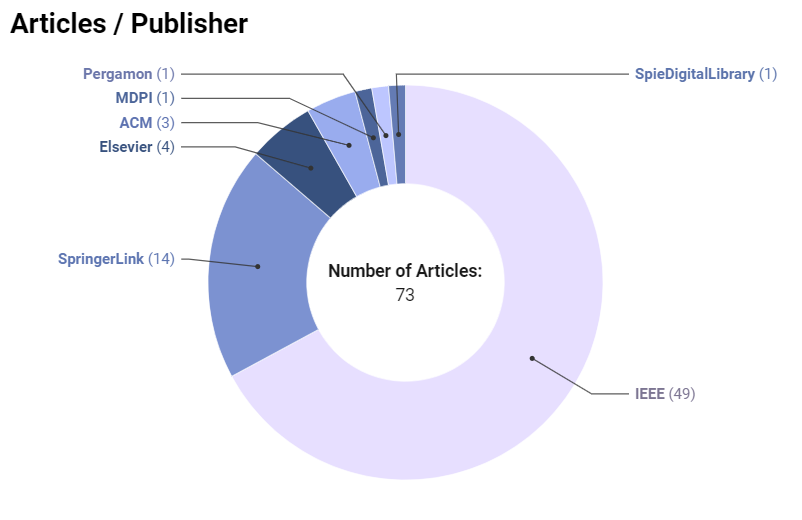
\includegraphics[width=\textwidth]{images/articles_per_publisher_2.png}
        % \includesvg[width=\textwidth]{images/svg/databases.svg}
    \end{subfigure}
    \begin{subfigure}[b]{0.45\textwidth}
    \caption{Number of selected papers per source.}
        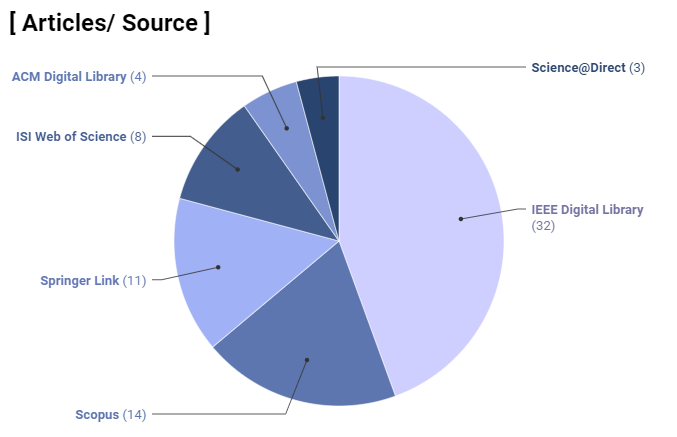
\includegraphics[width=\textwidth]{images/artpersrc_final.png}
        % \includesvg[width=\textwidth]{images/svg/itemtype.svg}
    \end{subfigure}
    \label{fig:archive-itemtype}
\end{figure}
 
Analysis of the distribution of selected papers based on publication year revealed that the majority of articles were published in 2022 and 2021 (see Figure \ref{fig:bar-chart-yaer}). Furthermore, the bar chart illustrates a general upward trend in the number of publications addressing security concerns for industries utilising Digital Twin and (I)IoT applications. This trend indicates that there is a growing interest and concern among researchers in the field of Digital Twin and (I)IoT security, and highlights the relevance of this systematic literature review.

\begin{figure}[H]    
    \caption{Yearly Publication Statistics: Investigating the Number of Papers Published}
    % \includesvg[width=0.9\textwidth]{images/svg/pub_year_white_bg.svg}
    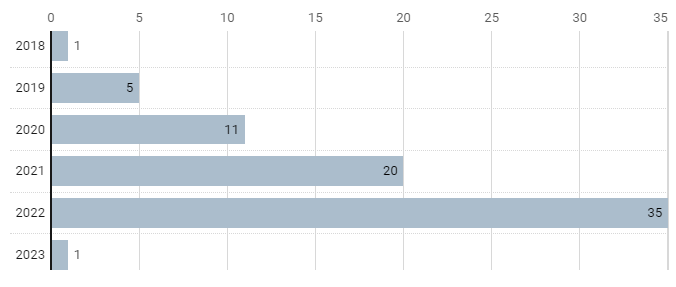
\includegraphics[width=\textwidth]{images/year8.png}
    \label{fig:bar-chart-yaer}
\end{figure}

To gain a deeper understanding of the trending topics within the 73 selected papers published between 2018 and 2023, a frequency analysis of keywords was conducted. This analysis was performed by extracting keywords that appeared more than three times in the abstracts and keyword sections of the articles using the VOSviewer tool. Further filtering and sensitization was applied to create a shortlist of keywords. Additionally, keywords which have similar meanings with different spellings and variations were merged. The resulting frequency analysis of keywords, illustrated in Figure \ref{fig:alluvial-key}, provides valuable insight into the key themes and concepts that are prevalent in current research on the topic of DT and IoT security. This analysis can help guide future research by identifying areas where there is a need for further investigation and providing a sense of the current state of the field.


\begin{figure}[H]
    % \includesvg[width=0.9\textwidth]{images/svg/key_buble.svg}
    % 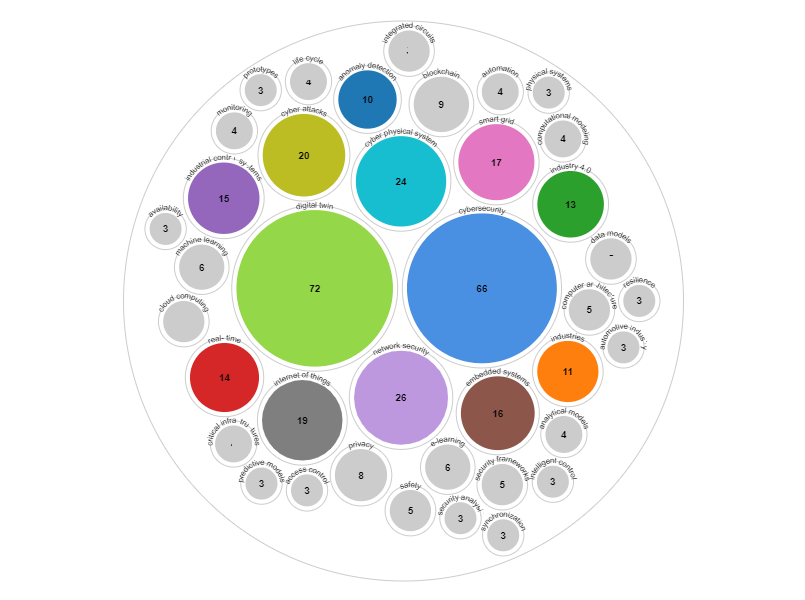
\includegraphics[width=\textwidth]{images/svg/key_buble.png}
    \caption{Frequency of keywords from abstract and keywords of 73 papers}
    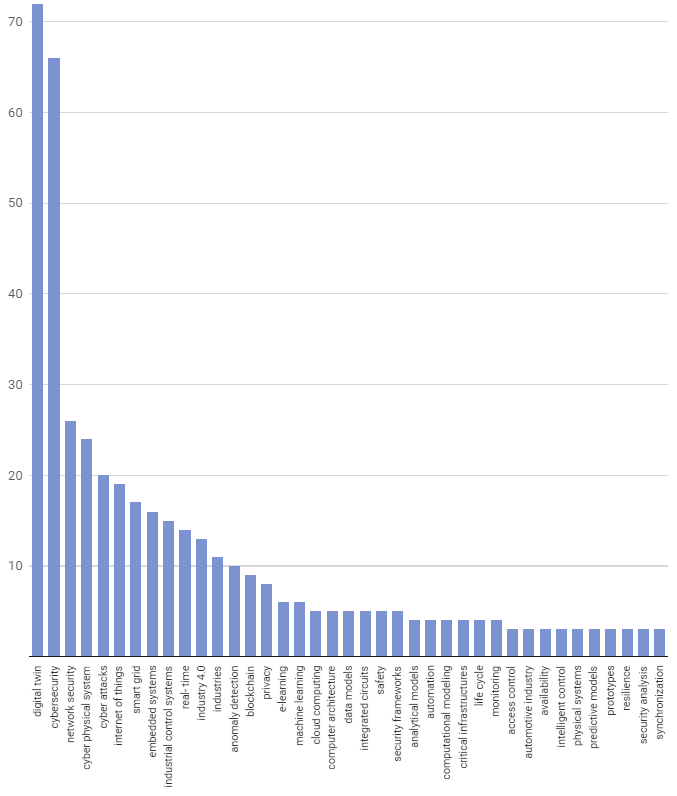
\includegraphics[width=0.8\textwidth]{images/keyword_occurance.png}
    \label{fig:alluvial-key}
\end{figure}
As was previous stated, in this study, 73 papers were analyzed to generate a list of 1187 keywords using VOSViewer. During our analysis, we utilized a thesaurus text file to merge keywords with similar semantic meanings.

For instance, we replaced artificial intelligence and deep learning with machine learning, and intrusion detection with anomaly detection. We also merged related terms such as cyber-attacks, denial-of-service attacks, cyber attacks, and computer crime into a single term - cyber attacks. Similarly, we combined control systems under the term industrial control system and grouped electric power transmission network and smart power grids as smart grid. We further streamlined our findings by using industry 4.0 as an umbrella term for smart manufacturing. Additionally, we have replaced the term "real-time system" with "real-time". 

Moreover, we limited the results to the top 87 keywords that appeared at least 3 times within the original list of 1187 keywords.  


The analysis of the selected papers using VOSviewer software revealed that which terms were frequently mentioned in the abstract and keyword section of the paper. The most frequently mentioned terms were "digital twin" with 72 occurrences, followed by "cybersecurity" with 66 occurrences, "cyberphysical system" with 24 occurrences, "cyber attacks" with 20 occurrences, "internet of things" with 19 occurrences, and "embedded systems" with 17 occurrences. This analysis highlights the key themes and concepts that are prevalent in current research on the topic of Digital Twin and IoT security. The high frequency of the term "digital twin" indicates the centrality of this concept in the field and the importance of understanding its role in ensuring the security of industries utilizing DT and IoT applications. The frequent mention of terms such as "cybersecurity" and "cyber attacks" further emphasizes the need for robust security measures to protect these systems from malicious actors. Additionally, the presence of terms such as "cyberphysical system" and "embedded systems" highlights the need for interdisciplinary research and collaboration between experts in fields such as computer science, engineering, and physics to effectively address the security challenges facing Digital Twin and IoT.

In order to gain further insights into the evolution of research in the field of Digital Twin and IoT security, a keyword co-relationship network analysis was extracted from the VOSviewer tool. This analysis aimed to identify clusters of related items and visualise the relationships between keywords over time. The results of this analysis revealed that in the early days of research on Digital Twin, keywords such as "monitoring", "safety", "prototypes", "resilience", "software", and "tools" were frequently mentioned, which suggests that the primary focus of research at that time was on utilising Digital Twin as a visual aiding tool. However, more recent research is characterized by the frequent mention of emerging technologies such as "blockchain," "machine learning," "e-learning" "5G," and "privacy" This indicates that the development of Digital Twin has shifted towards utilising these technologies and augment Digital Twin to provide more service other than used as a model.



\begin{figure}[H]
    % \centering    
    \caption{keyword co-relationship from VOSviewer}
    % 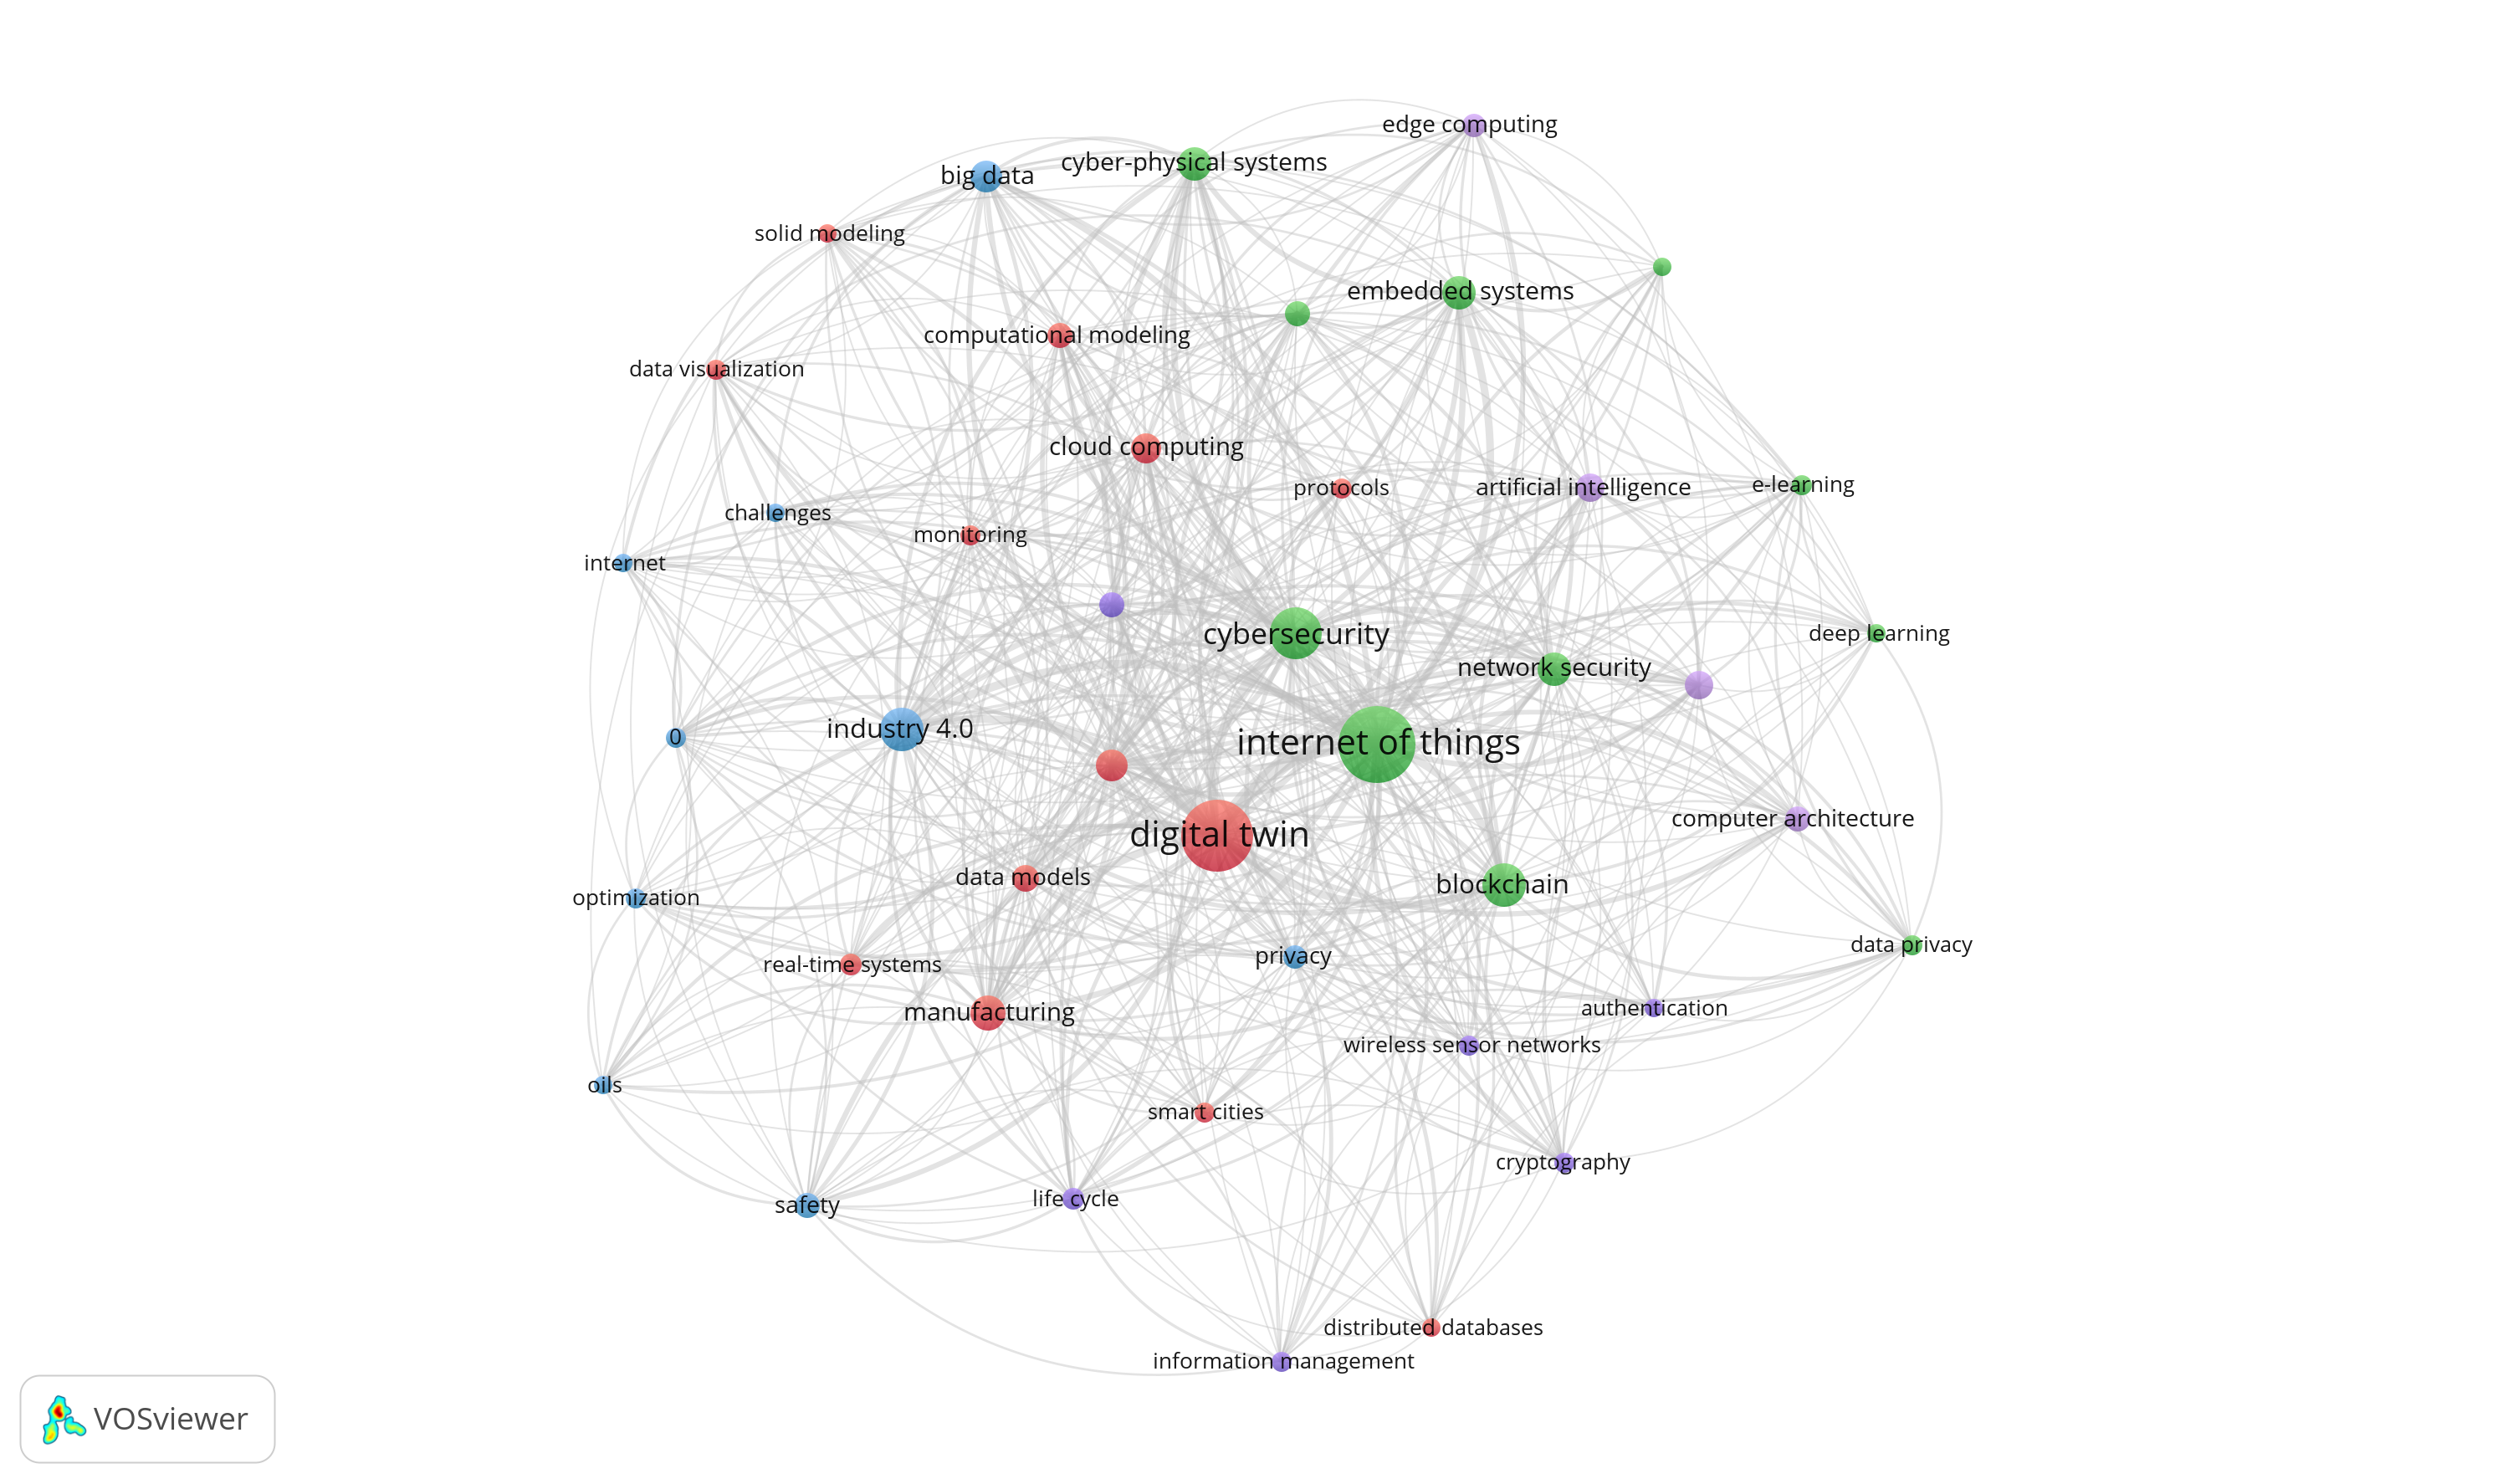
\includegraphics[width=1.5\textwidth, center]{images/vos_key_cooc_6_final.png}
    \includesvg[width=\textwidth]{images/svg/vos_co_time_2.svg}
    % \includesvg[inkscapelatex=false,width=0.95\columnwidth]{images/key_belt.svg}
    \label{fig:co-occurrence-vosv}
\end{figure}

The analysis of the co-occurrence of keywords in the selected articles, as represented in Figure \ref{fig:co-occurrence-vosv}, reveals the identification of five clusters. These clusters, as defined by the VOSviewer documentation, are groups of terms that exhibit a high degree of relatedness. 

Cluster one encompasses terms related to 5G technology, machine learning, real-time security analysis, security frameworks, access control, and automation highlighting the importance of incorporating advanced technologies in the field of security and access control automation. This cluster also suggests a growing emphasis on real-time security analysis to ensure quick identification and response to potential threats

Cluster two comprises keywords such as cybersecurity, data models, digital twin, internet of things, privacy, prototypes, safety, and cloud computing. The inclusion of terms such as privacy, prototypes, and safety in this cluster indicates a growing concern for the protection of sensitive information and the security of digital representations of physical systems. 

The third cluster encompasses terms such as those related to the automotive industry, availability, blockchain, industry 4.0, industrial control systems, system life cycles, intelligent control, software, and tools. This cluster suggests a growing emphasis on the use of blockchain technology for secure data management in the automotive industry for data sharing. 

The fourth cluster is comprised of analytical models, anomaly detection, cyber-attacks, monitoring, resilience, critical infrastructure, integrated circuits, and physical systems. This cluster shows the association of identification and mitigation of potential security threats through the use of analytical models to detect anomalies to increase the resilience of critical infrastructure.

The final cluster includes terms such as cyber-physical systems, e-learning, embedded systems, predictive models, and smart grids. This cluster highlight the importance of training and education to promote the secure use of cyber-physical system such as smart grids.
%----------------------------------------------------------------------------------------

% \subsection{Study Selection and Refinement}
%----------------------------------------------------------------------------------------
% ======================================================================================================
% NOTES, TODOS
% ======================================================================================================
\subsection{Study Selection and Refinement}
% 74 selected papers -> 14 not relevant and 3 duplicate studies submitted to different journals  excluded during full review of the papers. 

After the screening of 452 papers, initially, we were left with 89 papers. However, during the review phase, we exclude 21 papers from our analysis and data extraction. For example, we have found three studies that were duplicated with different metadata but had similar content and had been submitted to different journals. These duplicates were not identified by the tools we had used to exclude them. In addition, through the quality assessment checklist, we also excluded 18 papers for the data extraction phase.

Some of the reasons for the exclusion of these papers were as follows:

\begin{itemize}
    \item When the paper discussed how to secure the digital twin itself, rather than securing IoT applications using digital twin technology or securing the communication channel between DT and (I)IoT. 
    \item If the paper lacked a clear objective and aim.
    \item Some were not related to securing (I)IoT applications with an Industry 4.0 use case (for example, a study that used a digital twin to secure a data centre).
    \item Study sourced from book chapter. 
    \item The study was not relevant to any of the research questions.
    \item A study that focuses on securing (I)IoT devices that are not associated with any industry use case. 
\end{itemize}

As a result of this refinement and selection process, we were left with final set of 69papers that were used for data extraction and analysis. In the following chapter, we provide a review of the 69 papers focusing to answer two research questions: How is digital twin used to improve the security of (I)IoT applications and what security mechanisms are used to secure the communication channel?    




%----------------------------------------------------------------------------------------

% \subsection{Data Extraction and Monitoring}
%----------------------------------------------------------------------------------------
% ======================================================================================================
% NOTES, TODOS
% ======================================================================================================
% \subsection{Data Extraction and Monitoring}
\label{sec:data-ext}
%----------------------------------------------------------------------------------------

% \subsection{Data Synthesis}
%----------------------------------------------------------------------------------------
% ======================================================================================================
% NOTES, TODOS
% ======================================================================================================
% \subsection{Data Synthesis}
%----------------------------------------------------------------------------------------







%----------------------------------------------------------------------------------------

% Todo: Method for data extraction and synthensis 
% \subsection{Data Extraction Method}
% \subsection{Data Synthesis Method} 

% Chapter 3
% ======================================================================================================
% NOTES, TODOS

% ======================================================================================================

\chapter{Lightweight Cryptography Solution for (I)IoT-DT Communication}
\label{Chapter3} % For referencing the chapter elsewhere, use \ref{Chapter1} 



In the preceding chapter, the comprehensive examination of existing literature demonstrated that the majority of authors either presume the security of data transmitted from IoT sensors or recommend employing cryptographic methods like AES, SHA-256, and RSA to ensure a secure communication channel. However, applying such mechanisms on a resource-constrained device is unfeasible due to their substantial demands in terms of computation, memory, and power consumption \cite{vanderwalSecuringNetworksIoT2022a}

% In the previous chapter, the systematic literature review revealed that most of the authors either assume data communicated from IoT sensors are secure  or they suggest using AES, SHA-256, and RSA cryptography solutions to secure the communication channel. Implementing such mechanisms on a resource-constrained device however is impractical as these cryptographic solutions demand high resources in terms of computation, memory, and power . 



% The primary aim of this chapter is to respond to research question 3, which centers on enhancing the security of the communication channel between Digital Twin and resource-constrained (I)IoT devices. To tackle this issue, we present a proposed solution, which is a communication scheme involving the encryption of the data and authentication of the components using one of NIST's standardized lightweight algorithms known as ASCON.

The primary aim of this chapter is to respond to research question 3, which focuses on securing the communication channel between Digital Twin and resource-constrained (I)IoT devices. To address this challenge, we propose a solution (a communication scheme) that involves both encrypting and authenticating data communicated using one of NIST's standardized lightweight algorithms know as ASCON.  

Before diving into the implementation detail and the experiment outcome, we provide a background foundation for components and concepts relevant to the proposed solution in the following section. 



\section{Preliminaries}
% The following section was part of preliminary 
The implementation part of the proposed solution has four main components worth to describe them here. These are Digital Twin, (I)IoT devices, lightweight encryption algorithms, and MQTT protocol. This section serves as a foundation by providing background information for the aforementioned components.



\subsection{Digital Twin and Industry 4.0}
Digital Twin is an integrated software solution with modelling, analytical capability, and interconnectivity technology to replicate the physical world in digital space. The inception of this concept can be traced back to NASA's work on the Apollo 13 space project in 1970, where it was used as 'mirror systems' to troubleshoot and resolve issues \cite{adrienbacueDigitalTwinsEnhanced2022}. However, it was in 2002, the term "Digital Twin" coined for the first time by Michael Grieves and John Vickers of NASA in 2003, specifically for the application of product life cycle management \cite{jones_characterising_2020}.

The concept and definition of Digital Twins have been open to various interpretations, depending on the specific context.  However, through our systematic literature review in chapter \ref{Chapter2}, we identified Digital Twins typically revolve around three fundamental components: \textbf{states} (physical and digital), \textbf{interconnectivity} (communication channel between the physical and virtual state) and \textbf{process} (a mechanism for processing and analysing data). 

\begin{figure}[H]
    \centering
    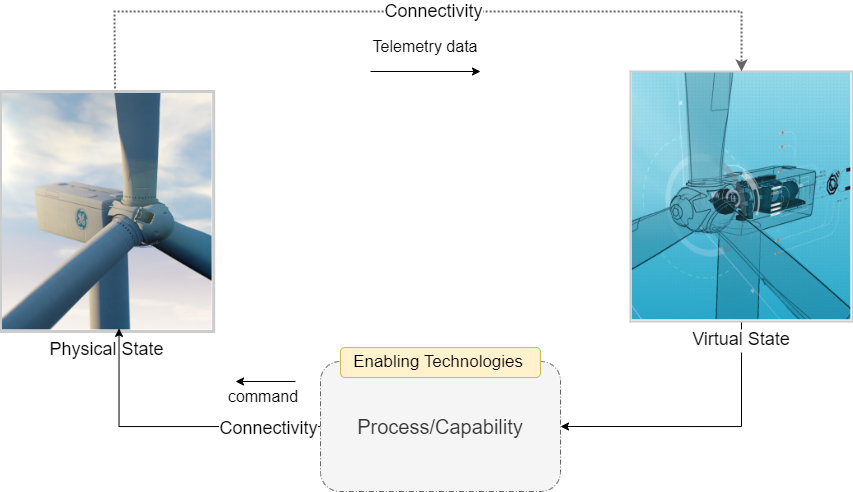
\includegraphics[width=1\linewidth]{images/fp/digital-twin-concept.drawio.png}
    \caption{Three Component of Digital Twin--State, Connectivity, and Capability(Process)}
    \label{fig:dt-concept}
\end{figure}

% Here, we provide a comprehensive definition of Digital Twin synthesised from a collection of various definitions of research publications:

% \textit{ Digital Twin is a virtual representation of a physical object, process or system that mirrors its real-world counterpart through real-time updates and tracking of its entire life-cycle. It is designed to model the physical characteristics and behaviours of the object using digital technology, mapping the physical operating environment to virtual space for interaction, and providing valuable insights through collecting asset-centric data, analytic capabilities, and simulations. Digital twins are used to monitor, simulate, optimise and predict the state of a physical object. They have a standard structure, end-to-end connectivity, communication protocol with backward compatibility, and a standard data format for communication between the twins.}

% The definition and respective reference are listed in Table \ref{tbl:dtconcept}


\begin{itemize}
% Virtual replica, Model, Evolving digital profile 
% A process, product, system, environment, industrial assest 
    \item \textbf{State}: Digit Twin has two states (see \ref{fig:dt-concept}); Virtual and Physical state. The virtual state is a digital (software) replica or model representation of a physical object, closely resembling the physical aspect. It can also be described as an evolving digital profile that captures the historical and current status of the represented object \cite{becueCyberFactorySecuringIndustry40with2018}. The physical state, on the other hand, refers to the real-world object of what the Digital Twin represents. The object that is represented by the virtual state could be physical components, processes \cite{wangDTCPNDigitalTwin2022, sousaELEGANTSecurityCritical2021, lopezDIGITALTWINSINTELLIGENT2021, rebecchiDigitalTwin5G2022, luongnguyenDigitalTwinIoT2022}, products, industrial assets \cite{dietzIntegratingDigitalTwin2020, eckhartEnhancingCyberSituational2019}, and environments.

    \item \textbf{Connectivity}: To keep the virtual state with the physical counterpart, a wired or wireless communication channel must be established. To keep the virtual state fidelity, the physical state should send  telemetry data (environmental sensor measurements) in real time. In this regard, wide sensor arrays can be deployed in the physical world to keep the data flow synchronized \cite{danilczykSmartGridAnomaly2021}. On the other hand, a command (a control message) can be sent from the virtual state to the physical state. Furthermore, ensuring a communication protocol that supports backward compatibility and adheres to a standard data format is required for achieving seamless data exchange between the two states \cite{atalayDigitalTwinsApproach2020}.

 
    \item \textbf{Process/Capability}: The true power of Digital Twin lies primarily due to the utilization of enabling technologies\cite{sousaELEGANTSecurityCritical2021}. This aspect also differentiates Digital Twin from simulation software. The use of enabling technology such as machine learning, blockchain, cloud computing, and big data analytics equipped Digital Twin with capabilities for better decision-making and to be used as a security tool. 
    
    Digital Twin can be equipped with enabling technology to provide various security services. For example,  detecting abnormal process events or deliberately injected malicious content \cite{saadImplementationIoTBasedDigital2020}, for prompt intervention and resolution of issues \cite{akbarianSecurityFrameworkDigital2021}, as a cyber situational awareness tool \cite{eckhartEnhancingCyberSituational2019} and so on.  
    
% In most definitions, Digital Twin is intended for simulation. One definition elaborates the simulation function as an insight gained through collecting asset-centric data. In quite a number of definitions, it is also stated that the digital twin is used for monitoring and controlling the real-world counterparts. In one definition the authors argued it can be used to increase cyber situational awareness for Cyber Critical Infrastructures


% In conclusion, Of the three core components of Digital Twin, only the "state" is explicitly described within the definition. The intended purpose and the interconnectivity between the two states are not always included in the provided definition.


    
\end{itemize}


% \begin{table}[H]
% \small
% \centering
% \caption{\label{tbl:dtconcept} Definition of digital twin in the literature}
% % \resizebox{\linewidth}{!}{
% \begin{NiceTabular}{p{10cm}|p{4cm}}
% \CodeBefore
% % \rowcolors[gray]{2}{0.8}{}[cols=1-2,restart]
% \Body
% \toprule
%     \textbf{DT definition} & \textbf{Reference(s)} \\
%     \midrule
%      Digital twins are virtual representations of industrial assets that provide valuable insights through collecting asset-centric data, analytic capabilities and simulations & \cite{dietzIntegratingDigitalTwin2020, eckhartEnhancingCyberSituational2019} \\  
%      \hline
%     A system that continuously monitors the physical state of an environment through wide sensor arrays and compares it to simulation models to gain deeper insights into its operating condition & \cite{williamdanilczykANGELIntelligentDigital2019, danilczykSmartGridAnomaly2021, veledarDigitalTwinsDependability2019, kumarBlockchainDeepLearning2022, hadarCyberDigitalTwin2020} \\
%     \hline
%     A virtual representation of a physical system, process or product that is synchronized with its real-world counterpart & \cite{gehrmann_digital_2020, luongnguyenDigitalTwinIoT2022, lopezDIGITALTWINSINTELLIGENT2021, rebecchiDigitalTwin5G2022} \\ 
%     \hline
%     A technology to map the physical operating environment to virtual space for interaction. & \cite{wuDeepLearningDriven2022}  \\ 
%     \hline
%     Evolving digital profile of the historical and current value of physical object or process & \cite{becueCyberFactorySecuringIndustry40with2018} \\
%     \hline

%     Virtual representation of physical objects or systems that can be used to monitor and control the real-world counterparts & \cite{almeaibedDigitalTwinAnalysis2021, chukkapalliCyberPhysicalSystemSecurity2021, dietzEmployingDigitalTwins2022}\\
%     \hline
%     virtual replica of physical object with standard structure, end-to-end connectivity, communication protocol with backward compatibility, and standard data format for communication between the twins & \cite{atalayDigitalTwinsApproach2020} \\

%     % \hline
%     % This paper is rejected
%     % DT is a mapping between physical object and virtual entity that receive data in real-time to predicate the state of the physical object & \cite{dinglingsuzehuiquDetectionDDoSAttacks2022} \\
    
%     \hline
%     A virtual Model designed to accurately map a physical object or process & \cite{wangDTCPNDigitalTwin2022, sousaELEGANTSecurityCritical2021} \\
    
%     \hline
%     a method to describe and model the physical characteristics and behaviors of physical objects by using digital technology & \cite{wangSoCbasedDigitalTwin2020} \\
    
%     \hline
%     A virtual space for representation of real world object and an information flow to keep them synchronize  & \cite{giovannipaolosellittoEnablingZeroTrust2021}\\
    
%     \hline
%     A digital twin is a virtual representation of a physical object that tracks and mimics its entire life-cycle through real-time updates & \cite{vargheseDigitalTwinbasedIntrusion2022, dietzUnleashingDigitalTwin2020} \\
    
%     \hline
%     Digital Twin is a virtual replica of physical system that precisely mirror the internal behavior of system for monitoring, simulating, optimizing and predicating the state of the system & \cite{akbarianSecurityFrameworkDigital2021, akbarianIntrusionDetectionDigital2020} \\
    
%     \hline
%     a digital twin is defined as an integrated system that combines computational, communication and physical aspects of Cyber Critical Infrastructures (CCIs) to provide increased cyber situational awareness & \cite{salviCyberresilienceCriticalCyber2022, pirbhulalNovelFrameworkReinforcing2022} \\
% \bottomrule
% \end{NiceTabular}
% % }
% \end{table}

% The definition presented in the table  \ref{tbl:dtconcept} is interpreted using the three components(State, Connectivity, Process) as follows.  


\subsection{Internet of Things and Industry 4.0 }
IoT and (I)IoT are related technologies where their difference relies only on their application area. While IoT is in IT and home environments,  IIoT is an application of IoT in the manufacturing industry \cite{boyes_industrial_2018}. In other words, it emerges from IoT \cite{fuller_digital_2020} to support the optimization of operations in industrial environments. Sensors, actuators and RFID are an instance of (I)IoT in the context of Industry 4.0. These technologies play a vital role in bridging the gap between the business IT environment and the operation environment in OT (operational technology) \cite{adrienbacueDigitalTwinsEnhanced2022}.


Though (I)IoT enhances control and visibility in industrial operations, it also introduces new attack surfaces as evidently shown by a study that reveals an increase in attacks like Stuxnet, flam, and Doqu on critical infrastructure as more SCADA systems communicate over TCP/IP communication channels \cite{eden_scada_2017}. And, Boyes et al. \cite{boyes_industrial_2018} point out that (I)IoT devices, such as sensors, actuators, and RFID tags, have limited power, storage, and processing capacity to support strong encryption mechanisms and effectively secure the communication channel. This is where our research contribution comes into play, addressing this challenge by implementing a lightweight cryptography-based communication scheme using a payload encryption technique.

\subsection{ESP31 - Wemos Lolin32 Lite}

The Wemos LOLIN32 Lite is a low-cost, low-power system on a chip (SoC)  microcontroller that is popular for Internet of Things (IoT) projects. It is based on the ESP32 SoC, which has a 32-bit dual-core processor, 4MB of flash memory, and 520kB of RAM \cite{noauthor_espressif_systems_01292021_esp32-1991551pdf_nodate}. The LOLIN32 Lite also has Wi-Fi and Bluetooth connectivity, making it ideal for this project as the implementation in this project involves sending and receiving data to and from Digital Twin through a wireless link. According to the datasheet of esp32 from espressive system, the board is low power consumption which can be used various application areas including industrial automation, health care and smart home \cite{noauthor_espressif_systems_01292021_esp32-1991551pdf_nodate}. 

The board is shipped with essential components for (I)IoT projects (see Figure \ref{fig:esp32}). At the centre, we have Xtensa microprocessors with 2 cores of 240 MHz clock frequency. It is equipped with 4MB of flash memory and it can also support external flash up 16MB. It has a number of GPIO (General Purpose Input/Output) pins for various functions. Among these, we leverage the GPIO 17 for data logging to an external power measurement unit (for further insights, refer to  Chapter \ref{Chapter4} Section \ref{sec:power})
Furthermore, two LEDs; one for the power charge indicator and the other for the GPI022 pin indicator are mounted. In addition, it supports USB connector for debugging and development with the help of UART CH340C USB-to-serial converter IC(Integrated Circuit).
\begin{figure}[H]    
{
    \centering
    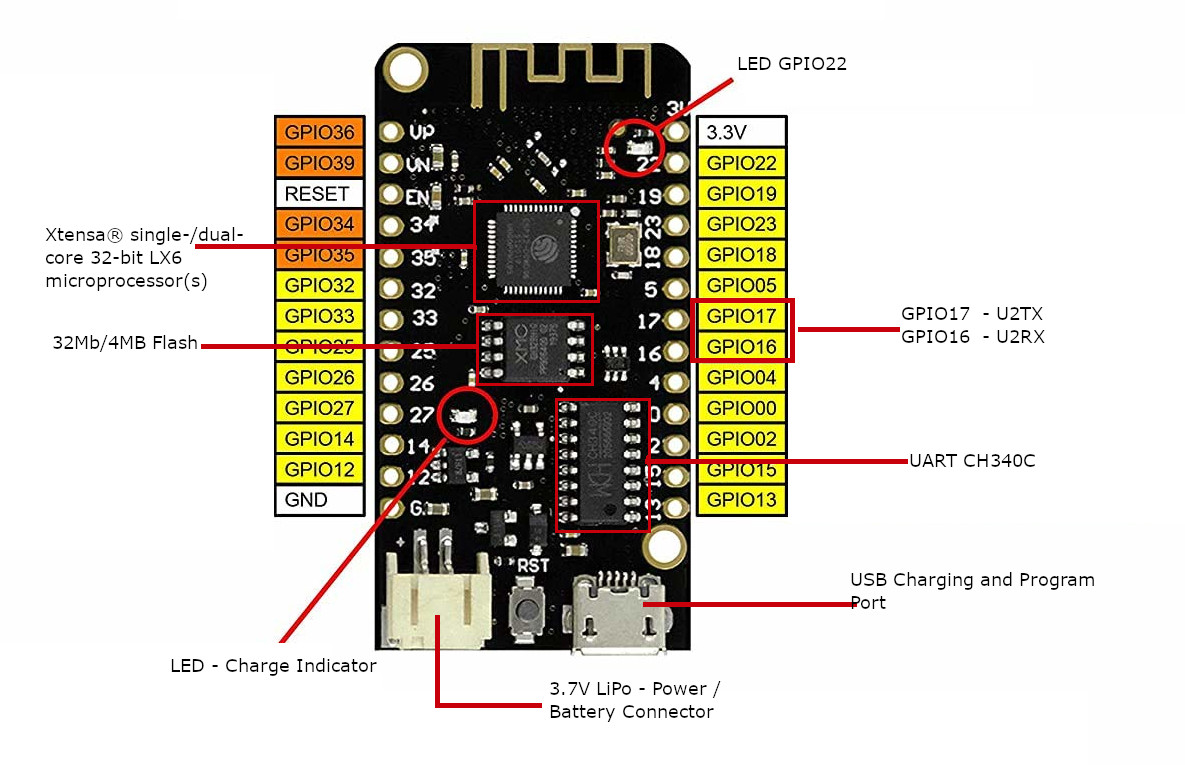
\includegraphics[width=0.99\textwidth]{images/fp/esp32final_edited.jpg}
    \caption{ESP32 Low-power Board From Espressif System}
    \label{fig:esp32}
}
\end{figure}

% \begin{table}[H]
%     % \tiny
%     \centering
%     \caption{\label{tbl:esp-spec} Technical Specification of Wemos Lolin32 Lite}
%     % \resizebox{\linewidth}{!}{
%     \begin{NiceTabular}{|p{2.5cm}|p{3cm}|}
%     \CodeBefore
%     % \rowcolors[gray]{2}{0.8}{}[cols=1-2,restart]
%     \Body
%     \toprule
%         Operating voltage &  3.3V \\
%         \hline
%         Supported Battery &	Lipo 3.7V\\
%         \hline
%         Battery Connector & PH-2 2.0mm\\
%         \hline
%         Digital I/O Pins & 22 \\
%         \hline
%          RAM Memory &  512KB\\
%         \hline
%         Clock Speed(Max) &	240MHz \\
%         \hline
%         SPI Flash &	4M Bytes \\
%         \hline
%         Size & 57*25.4mm \\
%     \bottomrule
%     \end{NiceTabular}
%     % }
% \end{table}

One of the key advantages of the Wemos LoLin32 Lite board is that it is supported by both the Arduino and ESP-IDF (Espressif IoT Development Framework) development environments. For our research project, we opted to use the Arduino embedded development framework to implement the ASCON and AES-GCM algorithms using the C and C++ programming languages. In addition, we utilized PlatformIO, an open-source platform for embedded development, to facilitate the building and deployment of our program onto the Wemos LoLin32 Lite board via the serial port.

\subsection{Lightweight Authenticated Encryption With Associated Data }


Lightweight Authenticated Encryption with Associated Data (AEAD) algorithms are designed to efficiently provide both confidentiality and message integrity in a single operation. These algorithms offer a balance between security and performance, making them suitable for securing data both at rest and in motion \cite{el-hajj_analysis_2023}. The confidentiality aspect is achieved through the generated cipher, while authentication or message integrity is ensured through the tag generated during encryption. Upon receipt, the receiver can decrypt the cipher to access the original message and simultaneously verify the tag to ensure that neither the message nor the cipher has been altered during transmission.

\subsubsection*{AES-GCM}

AES-GCM is a family of authenticated encryption with associated data based on AES (Advanced Encryption Standard) and GCM (Galois Counter Mode). It was first presented by David A. McGrew and John Viega \cite{mcgrew_galoiscounter_nodate} in 2005. Since then it has been adopted for various applications including for TLS and IPSec implementation \cite{salowey_aes_2008}.  


\subsubsection*{ASCON}

ASCON is an authenticated encryption algorithm designed and developed by Christoph Dobraunig, Maria Eichlseder, Florian Mendel and Martin Schläffer \cite{dobraunigAsconV1Lightweight2021}. It become very popular after it wins the CASEAR NIST computation. The authors claim the main goal of the algorithm is to provide simplicity, online, security, side-channel robustness, single-pass and lightweight cipher for the resource-constrained device \cite{dobraunigAsconV1Lightweight2021}. It is also a well-performing algorithm for short messages \cite{dobraunigAsconV1Lightweight2021} like for applications to collect environment and operating conditions in industry 4.0

The algorithm can also be used on high-performing machines to provide encryption and decryption for time-critical applications. It can provide 128-bit key security \cite{dobraunigAsconV1Lightweight2021}, surpassing the currently accepted 80-bit security standard.


\begin{figure}[H]
    \centering
    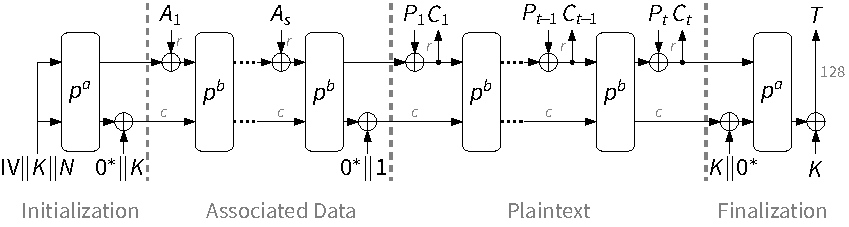
\includegraphics{images/fp/aead_encrypt.pdf}
    \caption{ASCON Encryption Mode of Operation (taken from \cite{dobraunig_ascon_nodate})}
    \label{fig:ascon-enc}
\end{figure}

The encryption and decryption process of ASCON is split into 4 main phases as depicted in Figure \ref{fig:ascon-enc} and \ref{fig:ascon-dec}. These are initialization, associated data processing, plain text/cipher text processing (depending on whether it is in encryption or decryption mod) and finalization. 



\begin{figure}[H]
    \centering
    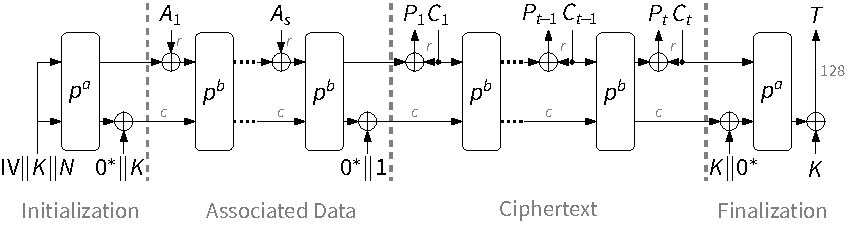
\includegraphics{images/fp/aead_decrypt.pdf}
    \caption{ASCON Decryption Mode of Operation (taken from \cite{dobraunig_ascon_nodate})}
    \label{fig:ascon-dec}
\end{figure}



\subsection{MQTT Protocol }
% What is MQTT
% Why it is important in the field of IoT and industry 4.0
% Key component of MQTT -> publisher, subscribers, and brokers
% lightweight nature of MQTT
% Asynchronous communication and real tim data transfer
% Security measures and authentication mechansims in MQTT

% use case and applicaiton of MQTT

% how we integrate lightweight encryption algorithm in MQTT
% limitation of MQTT

MQTT is a standard messaging protocol for the Internet of Things (IoT), designed and developed by Andy Stanford-Clark (IBM) and Arlen Nipper \cite{bryce_mqtt-g_2018}. It is an extremely lightweight publish/subscribe messaging transport that is ideal for constrained devices, such as microcontrollers and embedded computers \cite{andy_attack_2017}. MQTT is widely adopted in a variety of industries in IIoT systems, including automotive, manufacturing, telecommunications, oil, and gas \cite{atalayDigitalTwinsApproach2020}. 

MQTT protocol is not secure by design to safeguard and protect the data it carries over wire or wireless \cite{andy_attack_2017}. SSL can be used to encrypt the transport layer so that the MQTT header and message are secured. However, this additional security layer requires more resources which may not be available by device-constrained IoT devices. In this work, we show how to use this protocol to transmit an authentic and encrypted message using lightweight payload encryption without adding major additional overhead for the underlying device. 


\begin{figure}[H]
    \centering
    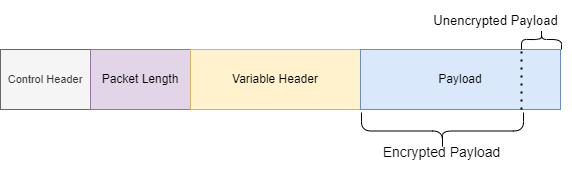
\includegraphics[width=\linewidth]{images/fp/mqttprotocol.drawio.png}
    \caption{MQTT Protocol Header Structure and Payload Encryption}
    \label{fig:mqtt}
\end{figure}

Figure \ref{fig:mqtt} shows the standard MQTT protocol header along with application message payload. Within the MQTT payload section, two distinctive parts can be identified. The first part consists of an encrypted message utilizing one of the AEAD (Authenticated Encryption with Associated Data) encryption family methods. For this particular study, both ASCON and AES-GCM encryption methods are implemented and compared. The second part of the payload contains the associated data. In this context, the device ID serves the purpose of retrieving the appropriate symmetric key by the receiver, thereby ensuring the message's authenticity and integrity.






% ------------------------------Note and Outline------------------------
% 
% The scheme should lightweight 
% The scheme should be secure enough 
% Provide both authentication and encryption 
%  
% 
% ------------------------------End------------------------


\section{Design Consideration and Requirement}
This section outlines the design consideration and requirements that guide the development of our proposed solution (communication scheme) for securing the communication between Digital Twin and (I)IoT. These considerations and requirements are defined primarily in consideration of the resource limitation of (I)IoT devices. 

\subsection{Design Consideration}
Our proposed solution is based on the following design choices that take into account the limited resource (I)IoT devices have.
\begin{itemize}
    \item The scheme should be based on the lightweight application protocol. 
    \item The underlying cryptographic algorithm should be based on a lightweight encryption algorithm standardized by NIST. 
\end{itemize}

\subsection{In Scope Requirements}
\textbf{Performance Requirement}: The proposed solution should be based on a cryptographic algorithm that performs better than traditional algorithms in terms of power consumption, speed, and storage complexity.

\textbf{Security Requirement}: The proposed solution should provide an adequate security level for typical data communication in Industry 4.0 environment. In this regard, an encryption algorithm that provides a minimum 80-bit security level (size of key) should be used. In addition to the above general security requirement, the proposed solution should provide the following security services. 
\begin{itemize}
    \item \textit{Message authentication}: The solution should enable the message receiver to check the authenticity of the message 
    \item \textit{Message Confidentiality}: The solution should provide message confidentiality by encrypting the message. 
    \item \textit{Data Integrity}: The solution should ensure the integrity of data transmission using checksums or other methods to detect message corruption.
    \item \textit{Resilience}: The solution should be capable of detecting man-in-the-middle attacks that involve message modification and data injection. 
\end{itemize}




\subsection{Out of Scope Requirements }
\begin{itemize}
    \item The proposed solution does not have a secure key exchange mechanism between Digital Twin and the physical device. In other words, symmetric keys are assumed to be pre-shared before communication starts. 
    \item The communication protocol (MQTT) at the application level is not encrypted using technologies like SSL/TLS to avoid computation overhead on the constrained device. 
    
\end{itemize}

% These design considerations and requirements are take into 
% proposed communication scheme should meet to be feasible to use in a real-world environment. 





\section{Proposed Solution  }
\label{sec:prosolution}

The (Industrial) Internet of Things ((I)IoT) devices are low-power and resource constrained, which makes them incapable of running traditional cryptographic
schemes such as AES, SHA-256 and RSA. Regardless, these devices are widely used across a range of Industry 4.0 sectors, such as manufacturing, transportation, health, and power
grids, for various applications. In addition, with the emergence of DT in Industry 4.0, (I)IoT sensors are an integral part of Digital Twin technology, in which they are used to collect and send data over wired or wireless channels. Hence, it is crucial to secure the communication between the DT and (I)IoT taking into consideration the limited resource they have. 


In this work, we proposed resource efficient communication scheme based on lightweight cryptographic authenticated encryption to enhance the security of the communication channel between the Digital Twin and its physical components over the MQTT protocol using a technique called payload encryption.


% \subsection{MQTT Payload Encryption/Authentication }

Payload encryption is a technique for ensuring message confidentiality at the application level. In other words, this approach can be used to establish an end-to-end secure channel between the sender and receiver at the application level to provide confidentiality over transmitted data. However, in this paper, we extend the scope beyond message confidentiality and introduce the use of the ASCON, a family of authenticated encryption with associated data (AEAD) algorithms, to provide both message authenticity and confidentiality.

Furthermore, we use the device ID as associative or additional data used along the key and plain text as input for the implementation of the ASCON algorithms. It is important to note that the device ID and its corresponding private key are assumed to be pre-shared between the communicating parties prior to initiating communication. In our case, while the device ID is managed and maintained by the Digital Twin device registration module, the symmetric key should be explicitly configured from both sides (Digital Twin and IoT) of the implementation.  

MQTT protocol is a lightweight messaging protocol that is often used in the Internet of Things (IoT) environment for communication at the application level. This protocol can be configured and programmed to support payload encryption using any encryption algorithm, including the ASCON and AES-GCM (family of AEAD based on AES). 

\begin{figure}[H]
   
    \centering
    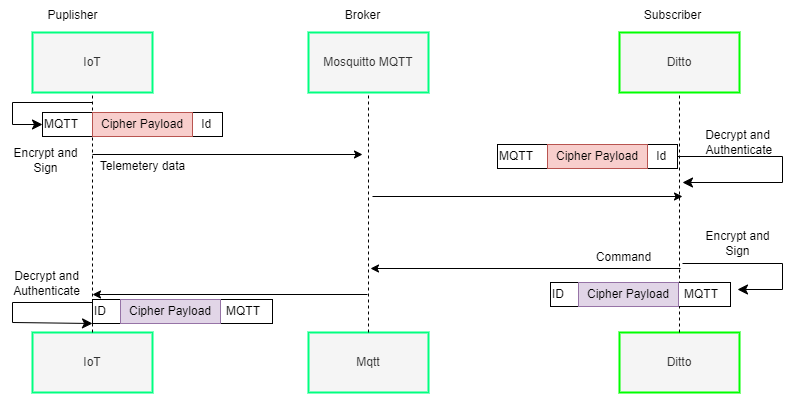
\includegraphics[width=\textwidth]{images/fp/payloadenc.drawio.png}
     \caption{Scheme of Payload Encryption With Authentication Over MQTT Protocol. }
    \label{fig:payload-encauth-schem}
\end{figure}

To achieve payload encryption using ASCON or AES-GCM algorithm over the MQTT protocol, the following steps should be taken. 
\begin{itemize}
    \item[-] \textit{Device ID registration}: Each connected device to Ditto should have a unique device ID. 
    \item[-] \textit{Generate and manage encryption keys}: The device and the Digital Twin agree on a symmetric key. 
    \item[-] \textit{Encrypting and Sending a message}: The sender encrypts the payload of the message along with a tag generated and publishes it to the MQTT broker. The associated data in this case is the unique ID of the device that is sending and receiving data to and from the Digital Twin. 
    \item[-] \textit{Forwarding or Proxing}: The MQTT broker proxies the message through the publisher-subscriber setting. 
    \item[-] \textit{Decryption and Authentication}: The receiver (subscriber) receives the MQTT message and decrypts the payload using a symmetric key retrieved using the device ID of the sender. The receiver then authenticates the payload to ensure that it is from the expected sender and that it has not been tampered with.
    
\end{itemize}

\textbf{\textit{End-To-End Payload Encryption and Authentication:}}
Our communication scheme is based on payload authenticated encryption using one of the AEAD (authenticated encryption with associated data) algorithms over the MQTT protocol. This Implicitly provides end-to-end confidentiality and integrity of a communicated message between Digital Twin and (I)IoT. The Mosquitto broker, which sits between Digital Twin and (I)IoT,  acts as a proxy for forwarding encrypted payload messages. Hence, only the communication parties are able to decrypt and authenticate the payload. 







\section{Implementation Approach}
To validate the applicability and efficacy of our proposed solution (based on lightweight cryptographic algorithms), we conducted an experiment using an ESP32 -- a resource-constrained IoT device -- and Ditto -- an open-source framework for building Digital Twin \footnote{https://eclipse.dev/ditto/}. We opt for ESP32 boards for the experiment due to the fact that they are low-cost and low-power devices in the market \cite{maier_comparative_2017}. Ditto was selected for its ease of customization through Java-based plugins and its widespread use in the open-source community. 



\begin{figure}[H]
    \centering
    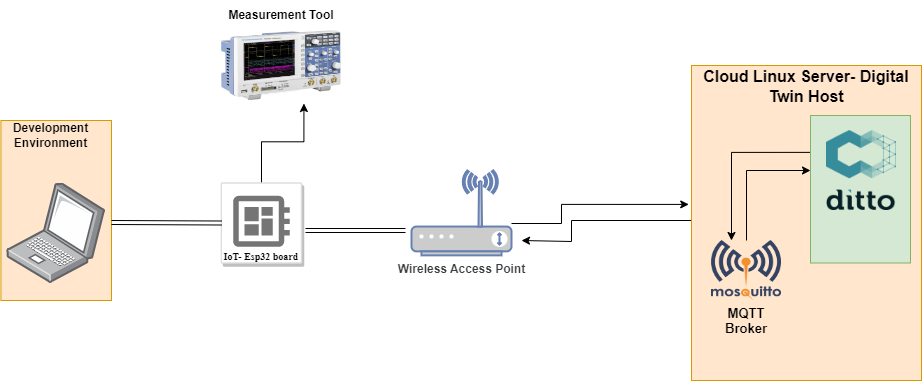
\includegraphics[width=\textwidth]{images/fp/experiment.drawio.png}
    \caption{Research Experiment Setup}
    \label{fig:experiment-setup}
\end{figure}

This section provides a detail of the experimental setup (of Fig \ref{fig:experiment-setup}) and implementation detail of the lightweight encryption/authentication algorithm implemented on both the constrained device and the Digital Twin framework.



% ======================================================================================================
% NOTES, TODOS
% What is Ditto -> reference the official webisite

% ======================================================================================================

\subsection{Eclipse Ditto - Digital Twin Setup}
Eclipse Ditto is an open-source framework for managing IoT devices to create Digital Twin \cite{noauthor_eclipse_nodate}.
It integrates devices via layers like Eclipse Hono and MQTT brokers, allowing managed Digital Twins to connect with various backend systems using protocols such as AMQP, Apache Kafka, HTTP, and MQTT. 

Ditto can be deployed on-premises or in the cloud. For this research, we build and deploy the Ditto code base in the cloud.
In addition, We have two options for deploying and running Ditto on a cloud Linux server. The first option involves utilizing the Kubernetes cluster, which necessitates substantial infrastructure resources. Specifically, a minimum of 4 GB RAM, 8 core processes, and 20 GB disk storage are required. However, the second option, which we have chosen, involves using Docker. This alternative demands fewer resources compared to the previous one. 

Running Ditto in a docker container have seven microservices operating in parallel, each fulfilling distinct functions. These microservices include \textit{Nginx} as the web server, \textit{}, \textit{Ditto Connectivity} for managing the device-to-Ditto connectivity, \textit{Ditto Thing} for managing things (counterpart of physical devices), \textit{Thing Search} for facilitating efficient search using MongoDB, \textit{Swagger-UI} for providing a web-based user interface, and \textit{Ditto Policies} for mainting controlled access over things.

The following steps outline the process required to set up Ditto on a Linux server:

\begin{itemize}
    \item \textbf{Install and Configure Docker:} Begin by installing Docker, a platform for creating and managing containers. Ensure Docker Compose, a utility for defining and running multi-container applications is also installed and configured on your Linux server.
    \item \textbf{Clone Ditto Codebase:} Access the official GitHub repository for Eclipse Ditto and clone the codebase using the command: git clone\texttt{https:// github.com/eclipse-ditto/ditto.git}. 
    \item \textbf{Deploy Ditto Microservices:} Start the Ditto cluster by deploying its microservices in containers. Execute the command: docker-compose up -d. 
    \item \textbf{Check Microservices Status:} verify that all microservices are running and check the health status of Ditto using the following commands: curl -u devops:foobar http://localhost:8080/status/health
\end{itemize}



The process of running Ditto and connecting with the MQTT broker is described below.

\textit{Creating Policy}: In Ditto policies are JSON configuration file that defines who access what. Creating policies is the first step in running Ditto. The policy configuration we use for our project is presented as follows. To speed up experimenting with Ditto we used a bash script that we can run from the terminal of the server. 
\begin{lstlisting}[style=CStyle, caption={A Bash Script of Ditto command To Create Connection}]
#!/bin/bash

curl -X PUT 'http://localhost:8080/api/2/policies/ut.thesis.demo:policy' -u 'ditto:ditto' -H 'Content-Type: application/json' -d '{
    "entries": {
        "owner": {
            "subjects": {
                "nginx:ditto": {
                    "type": "nginx basic auth user"
                }
            },
            "resources": {
                "thing:/": {
                    "grant": [
                        "READ","WRITE"
                    ],
                    "revoke": []
                },
                "policy:/": {
                    "grant": [
                        "READ","WRITE"
                    ],
                    "revoke": []
                },
                "message:/": {
                    "grant": [
                        "READ","WRITE"
                    ],
                    "revoke": []
                }
            }
        }
    }
}'
\end{lstlisting}

\textit{Creating things}: Things are the digital representation of the physical device with attributes and features. Like we did for policy, for the thing we also created bash script as follow. 

\begin{lstlisting}[style=CStyle, caption={A Bash Script To Create Things in Ditto}]
    

#!/bin/bash

curl -X PUT 'http://localhost:8080/api/2/things/ut-sensors:esp01' -u 'ditto:ditto' -H 'Content-Type: application/json' -d '{
    "policyId": "ut.thesis.demo:policy",
    "attributes": {
        "name": "Esp3201",
        "type": "Esp32 board"
    },
    "features": {
        "temperature": {
            "properties": {
                "value": 0
            }
        },
        "altitude": {
            "properties": {
                "value": 0
            }
        }
    }
}'
\end{lstlisting}

\textit{Creating connection:} The connection configuration file serves the purpose of defining the source and target of the MQTT broker topic. In this case, the connection type is MQTT, and the specified URI contains the IP address. The source topic is set as "ut-sensors/\#", indicating that Ditto will receive data from the broker when a message is published on any topic under "ut-sensors". On the other hand, the target address is defined as "ut-sensors/{{thing:id}}", which means that Ditto will publish data on the corresponding topic of the device whenever an event is emitted by the thing with the given ID. The inclusion of "\#" at the end of the string signifies that messages can be received from any topic under "ut-sensors". This configuration enables bidirectional communication and data exchange between Ditto and IoT devices via the MQTT broker. 

\begin{lstlisting}[style=CStyle, caption={A Bash Script to Create Connection in Ditto}]
#!/bin/bash

curl -X POST 'http://localhost:8080/devops/piggyback/connectivity?timeout=10' -u 'devops:foobar' -H 'Content-Type: application/json' -d '{
    "targetActorSelection": "/system/sharding/connection",
    "headers": {
        "aggregate": false
    },
    "piggybackCommand": {
        "type": "connectivity.commands:createConnection",
        "connection": {
            "id": "ascon-ut-mqtt-connection",
            "connectionType": "mqtt",
            "connectionStatus": "open",
            "failoverEnabled": true,
            "uri": "tcp://<IP address>:1883",
            "sources": [{
                "addresses": ["ut-sensors/#"],
                "authorizationContext": ["nginx:ditto"],
                "qos": 0,
                "filters": [],
                                "headerMapping": {},
                                "payloadMapping": ["AsconPayload"],
                                "replyTarget": {
                                        "headerMapping": {},
                                        "expectedResponseTypes": [
                                          "response",
                                          "error"
                                        ],
                                        "enabled":false
                                }
            }],
                        "targets": [{
                                "address": "ut-sensors/{{ thing:id }}",
                                "topics": [
                                "_/_/things/twin/events",
                                "_/_/things/live/messages"
                                ],
                                "authorizationContext": ["nginx:ditto"],
                                "headerMapping": {},
                "qos": 0,
                "payloadMapping": ["AsconPayload"]
                        }]
        }
    }
}'
\end{lstlisting}


Another crucial component that works hand in hand with Ditto is the MQTT broker. In the subsequent section, we will deep dive into the detailed process of setting it up and initiating its operation.

\subsection{Building MQTT Broker (Mosquitto) from Source}

The MQTT broker is a lightweight protocol designed for IoT communication[ref]. In our project, we utilized the MQTT implementation from Eclipse Ditto, specifically Mosquitto. To ensure full control and customization, we built the MQTT implementation from the source on our Linux server. This approach was undertaken primarily to accommodate the implementation of the lightweight encryption algorithm into the source code. However, we later decided to implement the algorithms by extending the ditto source code itself through the connectivity extension provided. 

In order to run the MQTT broker on our Linux server, there are a few necessary steps to follow. Firstly, we need to install a couple of dependencies, namely \texttt{libcjson-dev and libwebsocket-dev}. Once these dependencies are installed, we proceed to build the source code by executing the following command: 

\texttt{make WITH\_SRV=yes WITH\_TLS=no WITH\_WEBSOCKETS=yes WITH\_CJSON = yes WITH\_BUNDLED\_DEPS = yes WITH\_DOCS=no}. After the build process, we can verify the successful installation of MQTT by running the tests using the command \texttt{make test}. Finally, to complete the installation, we execute \texttt{sudo make install} to install the MQTT broker into our system. 


It is worth noting that the MQTT broker can be installed either on the same machine as the Ditto running machine or on a different remotely accessible machine. Our proposed scheme ensures secure communication between the IoT device and the cloud-hosted Ditto service. The MQTT broker has limited visibility, as it can only access the encrypted payload, thereby preventing any malicious broker from compromising the security of the communication. The lightweight authentication and encryption algorithm we leverage into our proposed solution guarantees the confidentiality and integrity of the data exchanged.

To start the MQTT service, there are two options available. The first option is to execute the command "mosquitto" directly. Alternatively, we can start the MQTT service with additional configuration options by specifying the configuration file path using the following command: "mosquitto -v -c /path/to/mosquitto.conf".

To publish and subscribe to topics using the MQTT broker, we utilize the commands provided on the GitHub page of Mosquitto. 
    \begin{itemize}
        \item For subscribing to a topic, we employ the command "mosquitto\_sub -t 'test/topic' -v". This command enables us to subscribe to the specified topic and receive the messages associated with it. 
        \item To publish a message to a topic, we run "mosquitto\_pub -t 'test/topic' -m 'hello world'". By executing this command, we can publish a message to the specified topic so that other subscribers to the topic get notified. 
    \end{itemize}
    
    
% \begin{figure}[H]
%     \caption{Ditto Architecture}
%     \centering
%     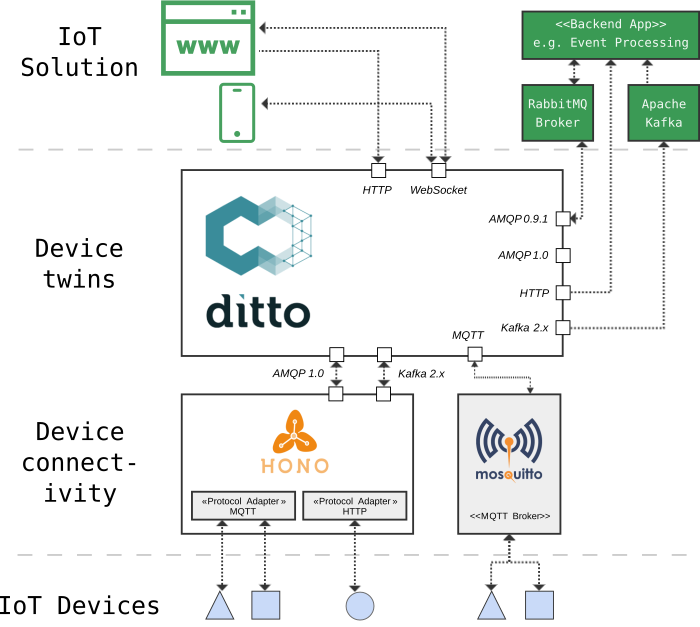
\includegraphics[width=\textwidth]{images/fp/ditto-overview-1.png}
%     \label{fig:ditto-arch}
% \end{figure}




\subsection{Implementation of ASCON and AES-GCM for device}


The implementation of both algorithms on the hardware IoT device was carried out using C and C++ programming languages within Arduino for esp-idf embedded development framework. We opted for C and C++ because those two choices are more suitable for low-level programming such as for embedded resource constraint devices. The main application for the IoT device was developed in C++, while the algorithm for ASCON and AES-GCM was implemented in C and incorporated through the use of the "extern" macro in C++ main application.


The counterpart of the algorithms in the digital twin was implemented in Java. This is because the connectivity microservice of Ditto is implemented in Java. This allowed us to extend the connectivity module using Java to incorporate an extension for encryption and decryption of the payload that comes from IoT devices.

It is worth noting that we neither altered nor introduced optimizations in the design of these algorithms. For both algorithms (ASCON\footnote{https://github.com/ascon/ascon\_collection} and AES-GCM\footnote{https://github.com/usnistgov/Lightweight-Cryptography-Benchmarking/tree/main /implementations/\_reference\_/crypto\_aead/aes-gcm/mbedtls}), we selected the optimized reference implementations tailored for the ESP32 device chip. However, to enhance the security of our implementation, we incorporated a function to generate a nonce. This aspect is crucial in addressing vulnerabilities such as replay attacks, which involve the repeated use of encrypted information.








\subsection{Ditto Java Base Payload Mapping}

In the context of Eclipse Ditto, data storage and transfer are facilitated through a format known as the Ditto protocol. This protocol utilizes a JSON structure, employing key-value pairs to represent and transmit information.

To seamlessly integrate with Ditto's capabilities, the connectivity microservice bundled with Ditto offers an extension specifically designed for intercepting incoming data. This extension allows for the mapping of data from its original form to a format that Ditto can understand and store in its underlying MongoDB database. Using the Ditto payload mapping feature, we can decrypt incoming encrypted payload messages and convert them into a format that Ditto can process and store.
 
With the payload mapping feature in Ditto's connectivity microservice, we can do the following: receive encrypted data from the IoT device, decrypt and authenticate it, and convert it into Ditto protocol messages. This helps ensure that the data sent between the IoT device and Ditto is secure and authentic.

To implement our custom mapping functionality to encrypt and decrypt, we perform the following steps:
\begin{itemize}
    \item[-] Implement and build a Java class as Jar file for the encryption and decryption functionality. This class will provide the ASCON or AES-GCM encryption and decryption operations needed for secure communication and data handling. 
    \item[-] Develop a custom message mapper class that will handle the conversion of incoming device messages to the appropriate Ditto protocol format. This class will integrate with the aforementioned encryption and decryption functionality to ensure data integrity and security during the mapping process.
    \item[-]Configure the Ditto connectivity microservice to recognize and load our custom message mapper. This configuration step ensures that incoming messages are routed to our custom mapper for processing, enabling seamless integration of our specific data transformation requirements within the Ditto framework.
\end{itemize}









\subsection{Sending Authenticated Encrypted Payload To Ditto}
\label{sec:sendingauth}

This section demonstrates the proof of concept securing the communication between the IoT device and the Digital Twin (Ditto). 

Figure \ref{fig:log-mon} depicts a snapshot captured from the serial monitor output of the board (device) utilizing PlatformIO (embedded development framework). The image showcases the device transmitting an encrypted payload to the 'ut-sensors' topic while including additional data labeled as 'tid' to uniquely identify the device. 

In Figure \ref{fig:wireshark}, a captured packet during the communication is displayed. Upon observation, it becomes evident that the topic being utilized is 'ut-sensors', and the message section of the MQTT protocol header contains the device identifier along with the encrypted payload.


\begin{figure}[H]
   
    \begin{subfigure}[c]{1\linewidth}
        \centering
        
        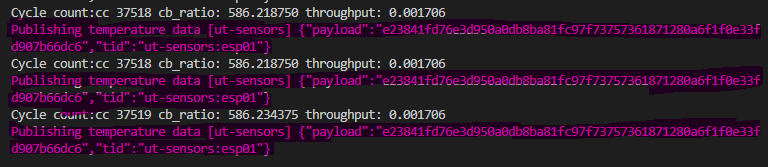
\includegraphics[width=\linewidth]{images/fp/serialport.png}
        \caption{Log Output of ESP32 Device Using Serial Monitor}
        \label{fig:log-mon}
     \end{subfigure}    

    \begin{subfigure}[c]{1\linewidth}
        \centering
        
        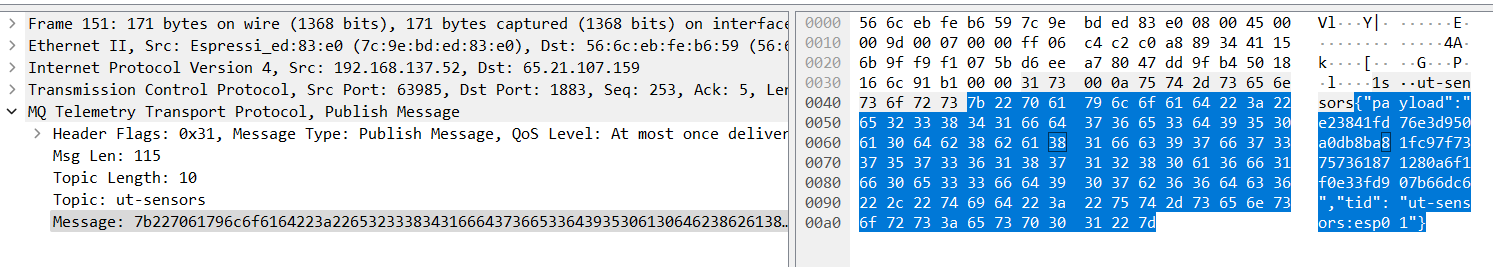
\includegraphics[width=\linewidth]{images/fp/wireshark.png}
        \caption{Wireshark Captured MQTT Communication From IoT to Ditto}
        \label{fig:wireshark}
    \end{subfigure}
     \caption{Serial Monitor of ESP32 Board and Wireshark Capturing Communication Between The Device and Ditto(DT)}
\end{figure}

The MQTT broker, hosted on the same server with Ditto, acts as a proxy, facilitating the transmission of authenticated and encrypted payloads through a publish-subscribe model. Once the MQTT broker receives a payload, it  notifies Ditto of the new message it has subscribed to. Ditto then retrieves the payload, decrypts it, and maps it into a Ditto protocol message, which is subsequently stored in a database.

To simulate the life cycle of a Digital Twin, we have developed a small web application that models the temperature and humidity features of an ESP32 sensor. The application utilizes JavaScript to retrieve these values through a stream of emissions using server-side events (SSE). Moreover, to send commands or messages to the server, we employ the HTTP POST API of Ditto. By subscribing to the command event associated with a specific topic, any device can consume the message and execute the corresponding action. This activity effectively simulates the communication between the digital twin and the actuators. Conversely, the communication from the (I)IoT device to the Digital Twin serves the purpose of collecting telemetry data from the operational environment.

\begin{figure}[H]
   
    \begin{subfigure}[c]{1\linewidth}
        
        \centering
        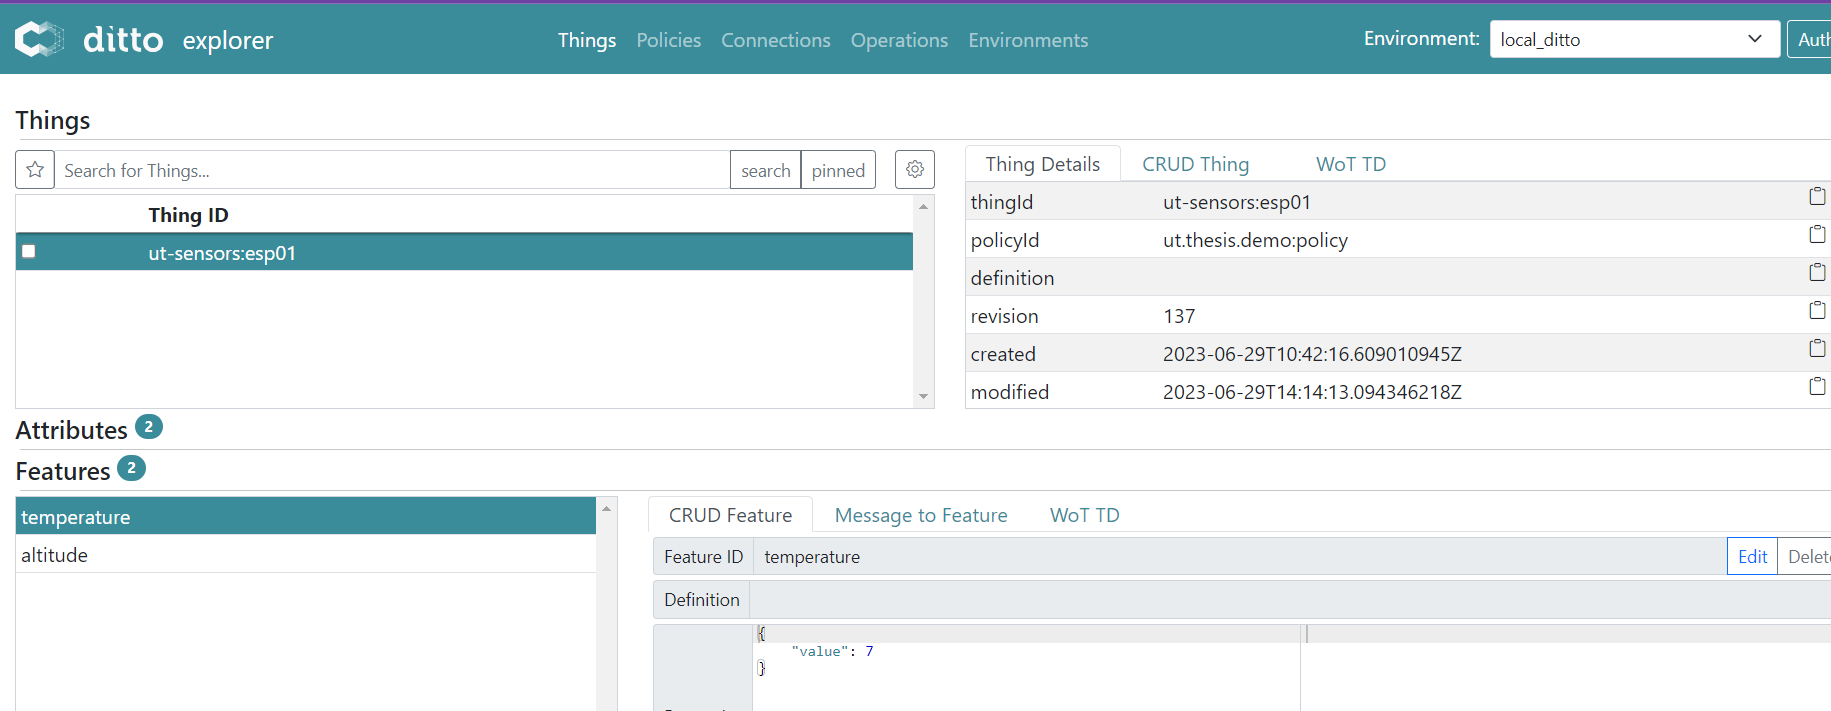
\includegraphics[width=\linewidth]{images/fp/ditto-log.png}
        \caption{A Data Log Viewed from Ditto Platform}
        \label{fig:ditto-log}
    \end{subfigure}
    
    \begin{subfigure}[c]{1\linewidth}
        \centering
        
        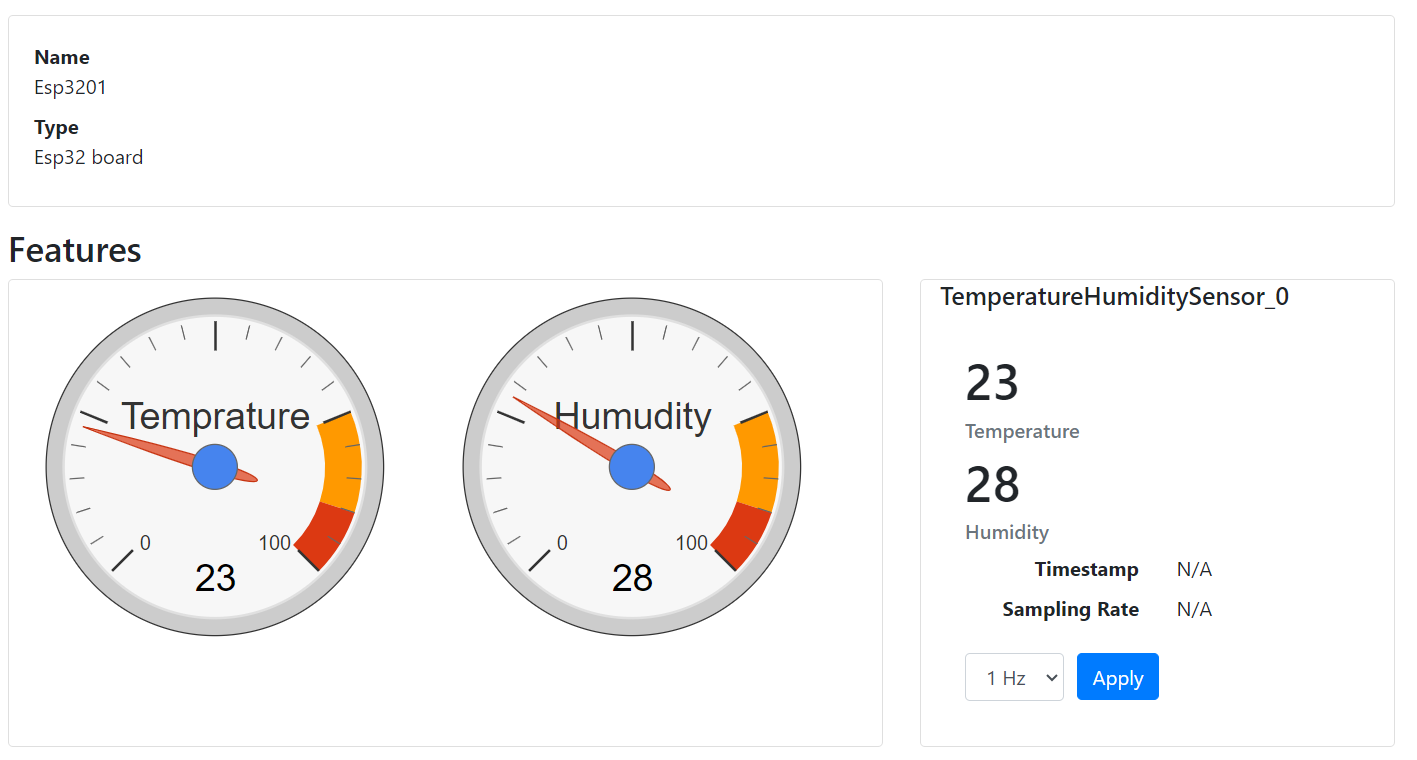
\includegraphics[width=\linewidth]{images/fp/appgauge.png}
        \caption{Web Application For Modeling Temperature and Humidity of ESP32}
        \label{fig:appdt}
     \end{subfigure} 
      \caption{Ditto and Webapp Toward Simulating Digital Twin}
    \label{fig:ditto-app}
\end{figure}

Figure \ref{fig:ditto-log} illustrates the WebUI of Ditto, which is included by default in the code base. This web portal serves as a portal offering device, policy, and connection management functionalities. Additionally, Figure \ref{fig:appdt} provides an overview of an application layer built on the Digital Twin concept. The attributes displayed on the upper part of the image represent the name and type of the simulated device. The gauges visually represent the received device features, while the bottom right section presents textual information associated with the device.

 
In this chapter, we discussed the relevant background information, the design requirement of the proposed solution and the implementation details. By implementing the proposed solution on both the Digital Twin (Ditto) and (I)IoT device (ESP32) we show how to secure the communication channel using a resource-efficient authenticated encryption algorithm. 

In the next chapter, we provided performance analysis results of our proposed solution in terms of speed, memory usage and power consumption. For the analysis, we measure the performance of three implementations which are without an encryption algorithm, with ASCON, the recent winner of NIST lightweight encryption competition, and AES-GCM, AES-based authenticated encryption with associated data algorithm. 






\include{chapters/chapter4} 

%----------------------------------------------------------------------------------------
%	THESIS CONTENT - APPENDICES
%----------------------------------------------------------------------------------------

\appendix % Cue to tell LaTeX that the following "chapters" are Appendices

% Include the appendices of the thesis as separate files from the Appendices folder
% Uncomment the lines as you write the Appendices

% % Appendix Template

\chapter{AppendixA: Proof of Concept Application Source Code } % Main appendix title

\label{AppendixA} % Change X to a consecutive letter; for referencing this appendix elsewhere, use \ref{AppendixX}

This appendix provides the main source code for the proof of concept application development based on our proposed solution. Note that, the source code for each encryption cryptography algorithm used in this paper is taken from the respective official GitHub repository. 

In addition, various lines of code are indicated and commented on to show how we perform measurements for latency, memory usage and UART logging for power analysis. 


\begin{lstlisting}[style=CStyle, caption={Main Source C File of The Proposed Implementation}, label={list:mainc-ascon}]

#include <Arduino.h>
#include <WiFi.h>
#include <sstream>
#include <iomanip>
#include <PubSubClient.h> // MQTT Client
// #include <time.h>
#include <esp_timer.h>
#include <esp_system.h>
#include <xtensa/core-macros.h>
// for generating nonce
#include <iostream>
#include <random>
#include <chrono>
// Libaries for UART
#include "driver/uart.h"
#include "driver/gpio.h"


extern "C" {
  #include "api.h"
  #include "core.h"
}

const char*  ssid         = "Linawifi";
const char*  password     = "Wifi3364";

const char*  mqtt_server  = "65.21.107.159";
const int    mqtt_port    = 1883;
const char*  mqtt_user    = "";
const char*  mqtt_pass    = "";


/*----------------------------------------------------------------------*/
// Define UART number for communication with the GPS.
/*----------------------------------------------------------------------*/
static const int RX_BUF_SIZE = 1024;

// Define TX and RX pins for the GPS.
#define TXD_PIN (GPIO_NUM_17)
#define RXD_PIN (GPIO_NUM_16)

// Define UART as number 2
#define UART UART_NUM_2


int num = 0;

/*----------------------------------------------------------------------*/



/*----------------------------------------------------------------------*/
// Function to generate random nonce of size 'size'
/*----------------------------------------------------------------------*/
std::string generateNonce(int size) {
    std::random_device rd;
    std::mt19937 gen(rd());
    std::uniform_int_distribution<> dis(0, 255);

    std::string nonce;
    for (int i = 0; i < size; ++i) {
        nonce += static_cast<char>(dis(gen));
    }

    return nonce;
}
/*----------------------------------------------------------------------*/


WiFiClient   wifi_client;
PubSubClient pubsub_client(wifi_client);


int encrypt_payload_ascon(unsigned char *p_cipher, unsigned char *payload, unsigned char *thingid){
     // Specify the size of the nonce you want to generate (in bytes)
    int nonceSize = 16; // Both ASCON and AES-GCM typically uses a 12-byte nonce
    // Generate a nonce
    std::string generatedNonce = generateNonce(nonceSize);

    // Convert the generated nonce to a const char array
    // const char nonce[] = "0123456789abcdef";
    const char *nonce = generatedNonce.c_str();

    unsigned char n[CRYPTO_NPUBBYTES]; 
    memcpy(n, nonce, sizeof(n));

    const char key[] = "thisismysymekey1";
    unsigned char k[CRYPTO_KEYBYTES];
    memcpy(k, key, sizeof(k));

    unsigned char *a = thingid;
    unsigned char *m = payload;
    // unsigned char c[32];

    unsigned long long alen = 16;
    unsigned long long mlen = 16;
    unsigned long long clen = CRYPTO_ABYTES;


    int result = 0;
    /* ======================= Cycle Count ======================= */
    // get esp cycle count
    // uint32_t StartCycleCount = xthal_get_ccount(); 


    /* ======================= Execution time ======================= */
    // //  Start the timer
    // uint64_t startTime = esp_timer_get_time();

    /* ======================= Memory Usage ======================= */
    // measure memory usage before the function call
    // uint32_t free_memory_before = esp_get_free_heap_size();
    // printf("Free memory before: %d bytes\n", free_memory_before);
    // Print the total heap size

    /* ======================= Function call ======================= */
    const char* logmsg = "[encrypt_payload_ascon] calling crypto_aead_encrypt-ascon.\n";
    uart_write_bytes(UART, logmsg, strlen(logmsg));
    result |= crypto_aead_encrypt(p_cipher, &clen, m, mlen, a, alen, (const unsigned char*)0, n, k);
    const char* logmsg2 = "[encrypt_payload_ascon] calling crypto_aead_encrypt-ascon.\n";
    uart_write_bytes(UART, logmsg2, strlen(logmsg2));

  
    /* ======================= End Cycle Count ======================= */
    // get endcyclecount using esp cycle count
    // uint32_t endCycleCount = xthal_get_ccount();

    // uint32_t cycleCount = endCycleCount - StartCycleCount;
    // size_t total_bytes = 64;
    // double cb_ratio = (double)cycleCount / total_bytes;
    // double throughput = (double)1 / cb_ratio;
    // // // print cycle count
    // printf("Cycle count:cc %u cb_ratio: %f throughput: %f\n", cycleCount, cb_ratio, throughput);
    
    
    /* ======================= End Execution time ======================= */
    // // Stop the timer
    // uint64_t endTime = esp_timer_get_time();
    // // Calculate the execution time
    // uint64_t executionTime = endTime - startTime;
    // // print execution time
    // printf("Execution time-alg: %llu microseconds\n", executionTime);

    /* ======================= End Memory Usage  Measureent=================== */
    // uint32_t free_memory_after = esp_get_free_heap_size();
    // // calculate the memory used by the function call
    // uint32_t memory_used = free_memory_before - free_memory_after;
    // // print memory used
    // printf("Memory used: %d bytes\n", memory_used);

    return result;
 }

unsigned char* const_char_to_unsigned_char(const char* p_str){
    // Input
    const char* str = p_str;
    size_t len = strlen(str);

    // Process
    // The following block of code is not secure as we are not considering to write null character at the end 
    // of the string.
    unsigned char* result = (unsigned char*)malloc(len);
    if(result != NULL){
        memcpy(result, str, len);
        // result[len] = '\0';
    }

    // Ouput 
    return result;
}

std::string float_to_string(float value) {
  std::ostringstream stream;
  stream << std::fixed << std::setprecision(2) << value;
  return stream.str();
}

std::string convertToHexString(const unsigned char* ptr, size_t size) {
    std::string hexString;
    hexString.reserve(size * 2); // Reserve space for the hexadecimal representation

    for (size_t i = 0; i < size; i++) {
        char hexBuffer[3];
        snprintf(hexBuffer, sizeof(hexBuffer), "%02x", static_cast<unsigned int>(ptr[i]));
        hexString += hexBuffer;
    }

    return hexString;
}

void publish_temperature_data(float value, float p_altitude) {
    // Construct topic string.
    std::string username(mqtt_user, 7);
    // std::string topic = "temperature/" + username + "/sensor";
    std::string topic = "ut-sensors";

    // Convert temperature to a string message.
    std::string tempstr = float_to_string(value);
    std::string altistr = float_to_string(p_altitude);

    const char payloadcc[] = "{\"tem\":7,\"al\":3}";
    unsigned char payloaduc[16]; 
    memcpy(payloaduc, payloadcc, sizeof(payloaduc));

    const char thingIdcc[] = "ut-sensors:esp01";
    unsigned char thingIduc[16];
    // Copy the string literal to unsigned char type variable 
    memcpy(thingIduc, thingIdcc, sizeof(thingIduc));

    unsigned char cipher[32];

    int result = 0;
    const char* logmsg = "[publish_temperature_data] calling encryption function-ascon.\n";
    uart_write_bytes(UART, logmsg, strlen(logmsg));
    result |= encrypt_payload_ascon(cipher, payloaduc, thingIduc);
    const char* logmsg2 = "[publish_temperature_data] end of encryption function call-ascon.\n";
    uart_write_bytes(UART, logmsg2, strlen(logmsg2));
    

    // std::string payloadEncr = encrypt_payload_ascon(payloadText,  );
    // "{\"payload\":\"bb6e50f539fbd657efe8021a19d101178289d87ccbc056348fd0d08fbc150528\",\"tid\":\"ut-sensors:esp01\"}"
    //{"payload":"e23841fd76e3d95682097eaafb38f7796fac95ed47e18bbb1ffd5f8d223e7a49","tid":"ut-sensors:esp01"}
    std::string payload = "{\"payload\":\"";
    // std::string payload_val = std::string(reinterpret_cast<char*>(cipher), sizeof(cipher));
    std::string payload_val = convertToHexString(cipher, 32);
    std::string tid = "\",\"tid\":";
    std::string tid_val = "\"ut-sensors:esp01\"}";

    std::string msg2 = payload + payload_val + tid + tid_val;

    // Serial.print("Publishing temperature data [");
    // Serial.print(topic.c_str());
    // Serial.print("] ");
    // Serial.println(msg2.c_str());
    // a1bd73dfea710f93e2782e50284d4c17a7be0d9a62114937fe34b2a32c16fae7
    // Publish!
    pubsub_client.publish(topic.c_str(), msg2.c_str(), msg2.length());
    // #MEM
    // printf("[publish_temparature_data]:Freep Heap Size Level 2 : %d bytes  minimum: %d bytes\n", esp_get_free_heap_size(), esp_get_minimum_free_heap_size()); 
}

void setup() {
  // Connect the board to wife access.
    Serial.begin(115200);
    WiFi.begin(ssid, password);
    delay(10000);


    // Initialize the UART connected to the GPS.
    const uart_config_t uart_config = {
        .baud_rate = 115200,
        .data_bits = UART_DATA_8_BITS,
        .parity    = UART_PARITY_DISABLE,
        .stop_bits = UART_STOP_BITS_1,
        .flow_ctrl = UART_HW_FLOWCTRL_DISABLE,
        .source_clk = UART_SCLK_APB,
    };

    // Install UART driver
    uart_driver_install(UART, RX_BUF_SIZE * 2, 0, 0, NULL, 0);
    uart_param_config(UART, &uart_config);
    uart_set_pin(UART, TXD_PIN, RXD_PIN, UART_PIN_NO_CHANGE, UART_PIN_NO_CHANGE);


    const char* test_str = "[Setup] Entering to main function.\n";
    uart_write_bytes(UART, test_str, strlen(test_str));

    // #MEM
    Serial.print("[setup]Total Heap Size First--->>: ");
    Serial.print(ESP.getHeapSize());
    Serial.println(" bytes");


    // Keep trying to reconnect if not connected yet.
    while (WiFi.status() != WL_CONNECTED) {
        delay(500);
        Serial.println("Connecting to WiFi...");
    }

    // Set up the mqtt server configuration.
    pubsub_client.setServer(mqtt_server, mqtt_port);
}

void reconnect() {
    // Loop until we're reconnected
    while (!pubsub_client.connected()) {
        Serial.print("Attempting MQTT connection...");

        // Attempt to connect
        if (pubsub_client.connect("", mqtt_user, mqtt_pass)) {
            Serial.println("connected");
        } else {
            Serial.print("failed, rc=");
            Serial.print(pubsub_client.state());
            Serial.println(" try again in 5 seconds");
            delay(5000);
        }
    }
}

void loop() {
    static int loopCounter = 0; 

    loopCounter++;

    
    // Get sensor values.
    float temperature = 9;
    float altitude = 4;

    // Reconnect if we lost connection.
    if (!pubsub_client.connected()) {
        reconnect();
    }
    // #MEM
    // printf("[loop]:Freep Heap Size Level 1: %d bytes  minimum: %d bytes\n", esp_get_free_heap_size(), esp_get_minimum_free_heap_size()); 

    if(loopCounter < 1000) {
        /* ======================= Execution time ======================= */
        // Start the timer
        // uint64_t startTime = esp_timer_get_time();

        /* ======================= RAM Memory Usage ====================== */
        // printf("[loop]:Freep Heap Size Level free: %d bytes  minimum: %d bytes\n", esp_get_free_heap_size(), esp_get_minimum_free_heap_size()); 


        // publish the sensor values 
        // *****************************************************************
        // ******************Function Call *****************************
        //
        printf("[loop]: Calling publish_temperature_data function-ascon.\n");
        publish_temperature_data(temperature, altitude);

        // 
        // ******************Function End ******************************
        //******************************************************************


        /* ======================= End Execution time ======================= */
        // // Stop the timer
        // uint64_t endTime = esp_timer_get_time();
        //  // Calculate the execution time
        // uint64_t executionTime = endTime - startTime;
        // // print execution time
        // printf("Execution time-app: %llu microseconds\n", executionTime);
    }

    // Update internal loops in mqtt client.
    pubsub_client.loop();


    // Wait for 2s before we read and publish the next sensor value.
    // Uncomment this line of code during power measurement 
    if (loopCounter % 100 == 0){
        delay(10000);
    }
    delay(500);
}
\end{lstlisting}

%% Appendix Template

\chapter{AppendixB:  } % Main appendix title

\label{AppendixB} % Change X to a consecutive letter; for referencing this appendix elsewhere, use \ref{AppendixX}

This appendix provides a code snippet that filters search results based on the presence of the term "digital twin" in the title of each paper. Specifically, the script used to extract search results from Springer Link. 


\begin{lstlisting}[language=Python, style=CStyle, caption={A python code snippet to identify papers which have "digital twin" in their title }, label={list:mainc-ascon}]

import csv

import re

 
counter = 0

results_file = '../data/SpringerLink_130523.csv'

accepted_filename = "../data/SpringerLink_130523_accepted.csv"

accepted_rows = []

 

with open(results_file, newline='', encoding="utf-8", errors="ignore") as fromfile:

    freader = csv.DictReader(fromfile, delimiter=';')

 

    for row in freader:

        counter += 1

        found = re.search(r'digital[\s-]{1}twin[s]?', row['Item Title'].lower())

 

        if found:

            accepted_rows.append(row)

 

with open(accepted_filename, 'w', newline='') as tofile:

    writer = csv.DictWriter(tofile, fieldnames=freader.fieldnames, delimiter=";")

    writer.writeheader()

    writer.writerows(accepted_rows)

 

print("count of papers:", counter)

print("count of papers with 'digital twin' in title:", len(accepted_rows))
\end{lstlisting}

%\include{Appendices/AppendixC}

%----------------------------------------------------------------------------------------
%	BIBLIOGRAPHY
%----------------------------------------------------------------------------------------

% \printbibliography[heading=bibintoc]
\printbibliography
%----------------------------------------------------------------------------------------
\end{document}